\documentclass[12pt,a4paper,twoside]{report}
\usepackage[utf8]{inputenc}
\usepackage[T1]{fontenc}
\usepackage[swedish]{babel}
\usepackage{amsmath}
\usepackage{ae}
\usepackage{units}
\usepackage{icomma}
\usepackage{color}
\usepackage{graphicx}
\usepackage{bbm}
\usepackage{textcomp}
\usepackage{url}
\usepackage{verbatim}
\usepackage{subfig}
\usepackage{marvosym}
\usepackage{eso-pic}
\usepackage{fancyhdr}
\usepackage{amssymb}
\usepackage{geometry}
\usepackage{titlesec}
\usepackage{boxedminipage}
\usepackage{cite}
\usepackage[table]{xcolor} % Färg i tabeller, använd exv \cellcolor{red}
\usepackage{xcolor}
\usepackage{listings}
\usepackage{mcode} % För m-filer, använd exv \lstinputlisting[firstline=5, lastline=15]{../code/FILENAME.m}

% åäö till comments i m-filer
\lstset{
  literate={ö}{{\"o}}1
           {ä}{{\"a}}1
           {å}{{\r{a}}}1
}

% Definiera bindestreck för math mode \mhyphen
\mathchardef\mhyphen="2D

% Omdefiniera paragraph kommandot med titlesec-paketet
\titleformat{\paragraph}[hang]{\normalfont\normalsize\bfseries}{\theparagraph}{1em}{}
\titlespacing*{\paragraph}{0pt}{3.25ex plus 1ex minus .2ex}{1em}

% -- Omdefiniera hur latex hanterar floats (figurer)
\renewcommand{\topfraction}{0.9}	
    \renewcommand{\bottomfraction}{0.8}	
    \setcounter{topnumber}{2}
    \setcounter{bottomnumber}{2}
    \setcounter{totalnumber}{4} 
    \setcounter{dbltopnumber}{2} 
    \renewcommand{\dbltopfraction}{0.9}	
    \renewcommand{\textfraction}{0.07}	
    \renewcommand{\floatpagefraction}{0.7}	
	% floatpagefraction MUST be less than topfraction !!
    \renewcommand{\dblfloatpagefraction}{0.7}
% --

%\linespread{1.3}
%\setcounter{secnumdepth}{-1}

\setlength{\headheight}{15pt}

\newcommand\BackgroundPic{
\numberwithin{equation}{section}
\put(-4,0){
\parbox[b][\paperheight]{\paperwidth}{
\includegraphics[width=\paperwidth,
keepaspectratio]{images/logo.eps}
\vfill
}}}

\setlength{\parindent}{0mm}
% Geometri på titelsida
\newgeometry{margin=0.5in}

\begin{document}
% Skapa "vattenmärke"
\AddToShipoutPicture*{\BackgroundPic}
\begin{titlepage}

\mbox{}
\vfill

% Bild på titelsidan?

\Huge
\textbf{Väderparametrars inverkan på \\energiförluster i en fastighet - \\en studie av värmeflöden}

\normalsize
% Teknisk Fysik?
\textit{Kandidatarbete inom civilingenjörsprogrammet Teknisk Fysik/Elektroteknik}

\vspace{1.5cm}

\large
Erik Ahlqvist\\
Ylva Dahl\\
Mats Lindström\\
Dan Ståby\\

\vspace{1cm}

\normalsize
Institutionen för Teknisk Fysik\\
CHALMERS TEKNISKA HÖGSKOLA\\
Göteborg, Sverige, 2012\\
% Vilket nummer har arbetet?
Kandidatarbete TIFX-02-12-19

\end{titlepage}

% Vilken indentation vill vi ha i texten?
\setlength{\parindent}{15pt}

\newpage
% Vilken geometri?
\newgeometry{margin=3cm, headheight=15pt}

%--- Sidhuvud & sidfot
	\pagestyle{fancy}
	\chead[\footnotesize Väderparametrars inverkan på energiförluster i en fastighet - en studie av värmeflöden]{\nouppercase{\footnotesize \leftmark}}
        \lhead[]{}
        \rhead[]{}
%---
	
\newpage
\thispagestyle{empty}
\mbox{}
\vspace{6cm}

\begin{center}
\large
KANDIDATARBETE TIFX-02-12-19\\
\vspace{1cm}
\Huge
Väderparametrars inverkan på \\energiförluster i en fastighet - \\en studie av värmeflöden\\
\vspace{1cm}
\normalsize
Kandidatarbete vid Teknisk Fysik\\
\vspace{1cm}
Erik Ahlqvist, Ylva Dahl, Mats Lindström, Dan Ståby\\
\vfill
Institutionen för Teknisk Fysik
\end{center}

\newpage
\pagenumbering{gobble}

\chapter*{Förord}

% Förord här

Vi vill rikta ett varmt tack till alla som har hjälp oss att möjliggöra detta projekt. 

Vi vill speciellt tacka Angela Sasic, lektor   på   Institutionen   för   Byggnadsteknologi   på   Chalmers, för att ha bistått oss med litteratur så väl som modeller, NN och NN, NÅGOT på SMHI för information om prognosstyrning av inomhusklimatet och sitt resonemang kring sådana modeller, NN, som generöst har delat sin datormodell med världen och tillåtit oss att NÅGOT.

Vidare vill vi tacka Peter Särneö, teknisk chef för fastigheten på Walleriusgatan, som ställt upp på möten och besvarat våra frågor, Peter Apell för korrekturläsning och många användbara kommentarer på små och stora texter, handledarna på Fackspråk som genom sin kunskap väglett och utbildat oss i processen kring att skriva en större rapport,

Avslutningsvis vill vi rikta ett stort tack till vår handledare Magnus Karlsteen som NÅGOT.

%\newpage


\section*{Sammanfattning}
% På svenska här

\newpage

\section*{Abstract}
% På engelska här

\newpage

\pagenumbering{roman}
\setcounter{tocdepth}{3} % Så att subsubsection syns i toc
\setcounter{secnumdepth}{3} % Numrerade subsubsections
\tableofcontents
\newpage

\pagenumbering{arabic}
\setcounter{page}{1}


%--- input går här:

% Inledning
\section{Inledning}

\subsection{Bakgrund}

Energi flödar hela tiden in och ut ur fastigheter, bland annat genom människors kroppsvärme, VVA (värme, ventilation och avlopp) och vädret ute. Dessa energiflöden kan delas in i konstanta energiflöden samt variabla energiflöden. Den främsta variabla energikällan är troligen vädret. Vädret kan, genom sina skiftningar, både ge och ta energi från byggnaden. För att bibehålla en jämn inomhustemperatur i fastigheten kan inte en konstant mängd energi tillföras av värmesystemet, utan energitillförseln måste hela tiden regleras utefter både konstanta samt variabla energiflöden.

I dagsläget regleras de flesta energisystem i fastigheter endast med tanke på utomhustemperaturen i varje ögonblick och på så sätt blir det alltid en fördröjning i uppvärmningen vilket i vårt fall leder till ojämn inomhustemperatur och eventuellt också till onödig energiåtgång.

Vår uppdragsgivare sköter utrustning för uppvärmning av fastigheten. Han har ett pågående projekt med syfte att minska energiförbrukningen i fastigheten samtidigt som ett behagligt inomhusklimat bibehålls. Inom ramen för detta så har en väderstation installerats på taket till fastigheten och sensorer av diverse slag har anslutits på strategiska platser.  Dessa enheter tillåter uppvärmningssystemet att anpassa energianvändningen efter väderlek.

Denna typ av effektivisering av energianvändningen i en fastighet är idag högaktuell på grund av höga energipriser och ökad förståelse för hur vår energianvändning kan påverka planeten negativt.


\section{Syfte}
Detta arbete syftar till att undersöka vilka energiförluster en fastighet har och hur dessa påverkas av olika väderrelaterade parametrar, som solinstrålning, utomhustemperatur och vind. Målet är att finna en kvanitativ beskrivning av hur energiflödena in och ut ur fastigheten påverkas av några olika väderparametrar. Primärt kommer vi att undersöka en fastighet på Walleriusgatan i Göteborg, men många av resultaten kommer att kunna appliceras även på andra byggnader.

Beskrivningen av hur vädret påverkar energiflödena skall sedan kunna leda till en modell för hur fastighetens reglerbara energiflöden ska kunna anpassas efter vädret så att en önskad inomhustemperatur bibehålls. I fastigheten som är associerad med projektet finns en väderstation monterad och det är ifrån den väderdata är tänkt att hämtas. Detta ska inte bara ge en trivsammare inomhusmiljö för de boende, utan även en energibesparing för fastigheten. Vi hoppas också kunna ge några byggnadstekniska förslag på åtgärder och kvantifiera hur stora besparingar detta skulle kunna ge – både energimässiga och ekonomiska.

Vi avser att främst bygga vår modell på att luften närmast fastigheten värms upp och bildar ett isolerande lager. Vi kommer också att ta hänsyn till både den fördröjning som sker i fastighetens väggar och den direkta uppvärmning och avkylning som sker med solinstrålning genom fönster respektive ofrivillig ventilation i form av drag.

På sikt hoppas vi att vårt arbete ska leda fram till ett modell som ger ett värde på hur mycket energi som behöver tillföras fastigheten i varje givet ögonblick, beroende på vilka värden väderstationen tidigare har tagit emot. I förlängningen ska detta kunna leda till energibesparande åtgärder för både den här och äldre fastigheter.

\section{Avgränsningar}

En detaljerad specifikation av värmeanläggningen och instruktioner för hur den ska drivas för att optimera energiförbrukningen kommer inte att ges i denna rapport. Troligen kan detta omfattas av ett eget kandidatarbete. Baserat på resultatet av detta arbete ska man däremot kunna bygga vidare mot en sådan tillämpning, med exempelvis dimensionering av ett reglersystem som följd.

Jämförelser med empiriska resultat har tyvärr inte varit möjligt då vi inte haft tillgång till nödvändig data, varken från väderstationen eller någon utomstående part.

Vi kommer också att bortse från oförutsägbara temperaturfluktuationer orsakade av exempelvis öppna fönster eller värmeeffekten från onormalt många människor i lägenheterna.



%Teori
\section{Teori}

För att beskriva fysikaliska fenomen används olika matematiska modeller. I våra simuleringar av vädrets inverkan på fastighetens energiflöden använder vi flera olika beräkningsmetoder. I det här avsnittet presenterar vi härledningar av de fysikaliska fenomen och beräkningsmetoder projektet använder sig av. Vi går också igenom definitioner av, för projektet, centrala begrepp.


\section{Värmeledning}
\label{sec:heatconduction}

Det pågår ständigt värmetransport från varma till kalla objekt. Konduktion, eller värmeledning, innebär att värmeenergi flödar genom ett material, utan att materialet i sig rör sig eller flyttar sig. Värmetransporten är proportionell mot temperaturskillnaden över konstruktionen. Konduktiviteten, eller värmeledningsförmågan, ofta betecknad $k$ inom fysiken eller $\lambda$ inom byggsektorn är en materialegenskap som beskriver hur snabbt en temperaturskillnad utjämnas genom konduktion i enheten $\unit{W~m^{-1}~K^{-1}}$. I denna rapport används den förstnämnda symbolen, $k$. För att bestämma $k$ för ett material utsätter man det för en temperaturskillnad och mäter den värmemängd som passerar genom materialet per tidsenhet. Generellt gäller att värmeflödet per ytenhet är $\mathbf{q} = - \unit[k \nabla T]{Wm^{-2}}$. Detta samband brukar kallas för Fouriers värmelag. I en dimension förenklas detta till

\begin{equation}\label{eq:conduction:fourier}\boxed{ \; \; \;
q_x = -k \frac{\mathrm{d}T}{\mathrm{d}x} \unit{Wm^{-2}}.
\; \; \; }
\end{equation}

Vid termisk jämvikt och homogent material kan detta utvecklas till

\begin{equation}
q_x = -\frac{k}{\mathrm{d}}\left( T_2-T_1\right) \unit{Wm^{-2}},
\end{equation}

där $d$ betecknar materialets tjocklek och $T_2$ samt $T_1$ är temperaturen i vardera änden av materialet. Begreppet U-värde kan nu införas och definieras som $U = \frac{k}{\mathrm{d}} \unit{Wm^{-2}K^{-1}}$, det vill säga $q_x = U\mathrm{d}T = U\left( T_2-T_1 \right)$. Även R-värdet introduceras och definieras som inversen av U-värdet, alltså $R=1/U \unit{m^2KW^{-1}}$. Observera att U- respektive R-värden endast kan användas vid termisk jämvikt, se härledningen nedan. Dessa två storheter är ofta användbara inom byggfysik och relaterade områden eftersom man med dem exempelvis kan jämföra olika väggars värmeledningsförmåga.

En schematisk bild över en vägg i en dimension som består av $n$ olika material kan ses i figur~\ref{fig:staticwallmethod:wall}. Med materialens värmeledningsförmåga, $k_i$, för $i=1,2\,,\,...\,,\,n$ samt längden på elementen, $d_i$, använder vi nu Fouriers värmeledningsekvation för att teckna värmeflödet och temperaturerna $T_i$, i punkterna mellan de olika delarna av väggen med randvillkoren $T_1 = T_H$ samt $T_{n+1} = T_L$.

\begin{figure}[hpbt]
\centering
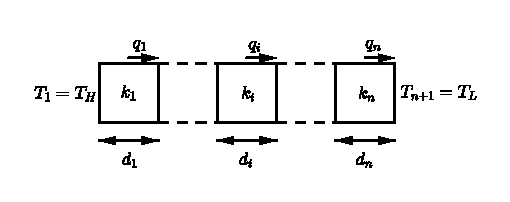
\includegraphics[scale=1.2]{images/wall.eps}
\caption{Schematisk bild över en vägg som består av $n$ olika element med olika
längd och värmeledningsförmåga.}\label{fig:staticwallmethod:wall}
\end{figure}

För varje del av väggen kan vi sätta upp ekvationer från Fouriers ekvation för värmeflöde. Vid termisk jämvikt blir flödet in i en del lika stort som flödet ut ur samma del vilket leder till att

\begin{equation}
\label{eq:staticwallmethod:rod}
q_i = -k_i\frac{T_{i+1}-T_{i}}{L_i} \, \Leftrightarrow \, \frac{L_i}{k_i}q_i = T_{i+1}-T_{i}
\end{equation}

Termisk jämvikt ger även att $q_1 = \, ... \, = q_i = \, ... \, = q_n$, vilket innebär att

\begin{equation}
\sum_{i=1}^n \frac{L_i}{k_i}q_i = q\sum_{i=1}^n \frac{L_i}{k_i} = q\sum_{i=1}^n R_i = \sum_{i=1}^n \left( T_{i}-T_{i+1} \right) = T_H - T_L 
\end{equation}

det vill säga

\begin{equation}
q R_\text{total} = T_H - T_L \Leftrightarrow q = U_\text{total} \left( T_H - T_L \right)
\end{equation}

där

\begin{equation}
U_\text{total} = \frac{1}{R_\text{total}} = \frac{1}{\sum_{i=1}^N R_i}.
\end{equation}

Värmeledningsförmågan, och därmed även R- samt U-värden, påverkas av materialets densitet, porositet, temperatur samt fuktighet. Fuktkorrigering görs ibland, enligt vissa framställda värden.

Utifrån Fouriers värmelag kan man härleda ytterligare ett viktigt samband, värmeledningsekvationen. Anta en infinitesimal volym, som varken utsätts för eller utför något arbete relativt omgivningen. Enligt grundläggande termodynamik kan då en godtyckligt liten förändring av värmeenergin (i $\unit{J m^{-3}}$) skrivas som $\mathrm{d}Q = c_p \rho \mathrm{d}T$.  I en dimension, över ett litet tidssteg $t-\mathrm{d}t< \tau < t+\mathrm{d}t$ och en liten sträcka $x-\mathrm{d}x < l < x+\mathrm{d}x$, fås att

\begin{equation}
\mathrm{d}E = c_p \rho \int_{x-\mathrm{d}x}^{x+\mathrm{d}x} \left[ T\left( l, t+\mathrm{d}t\right) - T\left( l, t-\mathrm{d}t\right)\right]dl = c_p \rho \int_{t-\mathrm{d}t}^{t+\mathrm{d}t} \int_{x-\mathrm{d}x}^{x+\mathrm{d}x} \frac{\partial T}{\partial \tau} \mathrm{d}l\mathrm{d}\tau
\end{equation}

Från Fouriers värmelag blir för samma förändring

\begin{equation}
\mathrm{d}E = k\int_{t-\mathrm{d}t}^{t+\mathrm{d}t} \left[ \frac{\partial T}{\partial x}\left( x + \mathrm{d}x, \tau \right) - \frac{\partial T}{\partial x}\left( x-\mathrm{d}x, \tau \right)\right]d\tau =  \int_{x-\mathrm{d}x}^{x+\mathrm{d}x} \frac{\partial}{\partial x} \left( k \int_{t-\mathrm{d}t}^{t+\mathrm{d}t} \frac{\partial T}{\partial x} \mathrm{d}\tau \right)\mathrm{d}l
\end{equation}

Kombinering av dessa och det faktum att det gäller för en godtycklig sträcka $\mathrm{d}l$ samt tid $\mathrm{d}\tau$, vilket innebär att integralen kan tas bort, ger att

\begin{equation}\label{eq:conduction:heateq}\boxed{ \; \; \;
c_p \rho \frac{\partial T}{\partial t} = \frac{\partial}{\partial x} \left( k \frac{\partial T}{\partial x} \right) \Leftrightarrow \frac{\partial T}{\partial t} = \alpha \Delta T
\; \; \; }
\end{equation}

där det andra sambandet gäller då $k$ är oberoende av $x$. Detta samband brukar kallas för värmeledningsekvationen.

\paragraph{Tröghet}
Det kan förefalla intuitivt att väderförändringar påverkar fastigheter, men hur mycket det spelar roll det egentligen? I det resonemanget spelar termen tröghet en betydande roll. Beroende på hur tjocka väggarna är, samt vilket material de är byggda av spelar de yttre omständigheterna olika stor roll. Trögheten i väggarna är således ett begrepp för hur lång tid det tar innan en väderförändring märks inomhus då yttre parametrarna ändrar sig. En stor tröghet bidrar till ett jämnare inomhusklimat då väggarna fungerar som lågpassfilter och dämpar svängningarna i temperaturen.

\section{Svartkroppsstrålning}
\label{sec:blackbody}

Alla objekt reflekterar, absorberar eller transmitterar ljus. De kroppar som varken 
reflekterar eller transmitterar något ljus utan absorberar $\unit[100]{\%}$ kallas konventionellt för svartkroppar. Detta är dock en teoretisk konstruktion då perfekta svartkroppar inte existerar men modellen kan ändå användas som en god modell i flera fysikaliska 
tillämpningar. Den energi som absorberats av kroppen strålas ut i form av svartkroppsstrålning vars 
frekvensspektrum bestäms av kroppens temperatur när kroppen är i termisk jämvikt med
 sin omgivning. Den totala utstrålade energin per tidsenhet fås ur Stefan-Boltzmanns lag
 
\begin{equation}
\label{eq:boltzmanslag}
\boxed{ \; \; \;
j^{\star} = \sigma T^{4}
\; \; \; }
\end{equation}

\noindent
där $\sigma$ är Stefan-Boltzmanns konstant som mäts i $\unit{W~m^{-2}~K^{-4}}$ och $T$ är kroppens temperatur vid termisk jämvikt.

\subsection{Härledning}
% av stefan-boltzmanns lag
% med hål i en låda
% kolla i termoboken
I en låda med fotoner kan den totala energin inne i lådan beskrivas som 
\begin{equation}
\label{eq:photonbox}
\frac{U}{V}=\frac{8\pi^5}{15}\frac{(kT)^4}{(hc)^3}
\end{equation}

där $U$ är  och $V$ är lådans volym. Ekvationen fås ur Plancks spektrum.\cite[ss.~301-302]{schroeder00} % Ev. förtydliga mer om vad som fås ur Plancks spektrum och vad U är.

Sedan görs ett litet hål i lådan, så att några av fotonerna kan slippa ut. Sannolikheten för att fotoner med kort respektive lång våglängd ska slippa ut är densamma som fördelningen mellan dem inne i lådan, eftersom de har samma hastighet.

Den totala mängden strålning som kommer ut kan då beräknas genom att tänka sig att 
de fotoner som når fram till hålet under en kort tidsperiod, $\mathrm{d}t$, alla befann sig
 på samma hemisfäriskt skal inne i lådan för en liten stund sedan, se figur \ref{fig:box}. Tjockleken på detta tänkta hemisfäriska skal är $c\mathrm{d}t$. Hemisfärens radie, $R$, beror givetvis på hur långt bakåt i tiden vi tittar.

\begin{figure}[hpbt]
\centering
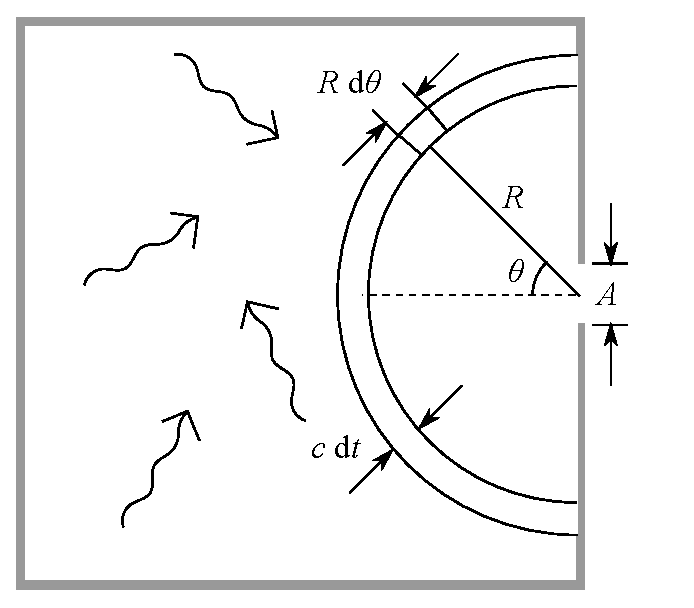
\includegraphics[height=5cm]{images/blackbody_box.eps}
\caption{\label{fig:box}{Fotonerna som lämnar lådan har en liten stund tidigare befunnit sig i samma hemisfär inne i lådan.}}
\end{figure}


Ett volymelement av det hemsfäriska skalet ges av
\begin{equation}
V=(R\mathrm{d}\theta) \times (R\sin\theta\mathrm{d}\phi) \times (c \mathrm{d}t).
\end{equation}

Energitätheten för fotonerna i volymelementet är således
\begin{equation}
E_\text{v.e.}=\frac{U}{V} c \mathrm{d}t R^2 \sin\theta \mathrm{d}\theta \mathrm{d}\phi.
\end{equation}

Men endast den andel av fotonerna som har rätt riktning kommer ut genom lådans öppning. Sannolikheten för att en foton har rätt riktning är
\begin{equation}
P(\text{rätt riktning})=\frac{A\cos\theta}{4\pi R^2}
\end{equation}

där A är hålets area. Den totala energin som strålar ut ur hålet från det lilla 
volymelementet är alltså 
\begin{equation}
\frac{A\cos\theta}{4\pi}\frac{U}{V} c\mathrm{d}t \sin\theta\mathrm{d}\theta \mathrm{d}\phi
\end{equation}

vilket ger en total energiutstrålning på
\begin{equation}
\frac{A}{4}\frac{U}{V}c \mathrm{d}t.
\end{equation}

Givetvis är utstrålningen beroende av både hålets area och tidsintervallet. Dividerar vi med dessa storheter får vi effekt per ytenhet, $j$,
\begin{equation}
j=\frac{c}{4}\frac{U}{V}. 
\end{equation}

Sätt in detta uttryck i ekvation~\eqref{eq:photonbox} så fås det vi känner som Stefan-Boltzmans lag,~\eqref{eq:boltzmanslag}
\begin{equation}
j=\frac{2\pi^5}{15}{(kT)^4}{h^3c^2}=\sigma T^4
\end{equation}

där $\sigma=\frac{2\pi^5k^4}{15h^3c^2}$ är Stefan-Boltzmans konstant.


\subsection{Strålning från omgivningen}
\label{sec:bb_sur}

\begin{figure}[hpbt]
\centering
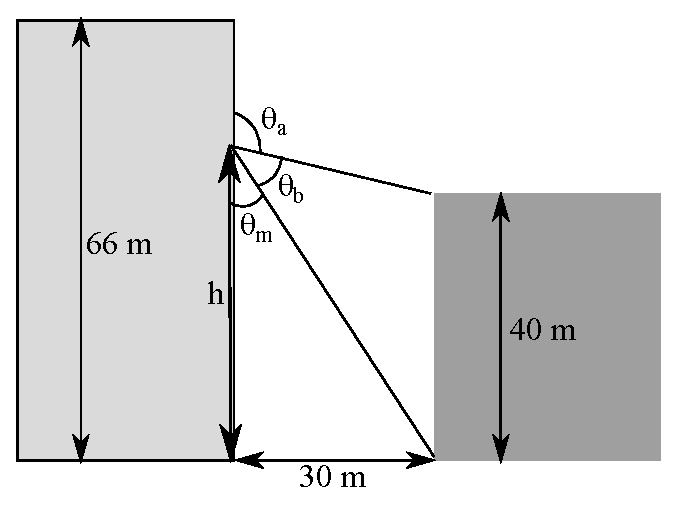
\includegraphics[height=4cm]{images/blackbody_surroundings.eps}
\caption{\label{fig:surroundings}{Den undersökta fastigheten på 
Wallerius\-gatan till vänster, och Johannebergs\-kyrkans församlings\-hem till höger. Den mot väggen instrålade svartkroppstrålningen kommer från olika källor. Här illustreras hur mycket av väggens omgivning som upptas mark, annan fastighet respektive atmosfären.}}
\end{figure}

För att uppskatta hur mycket svartkroppsstrålning som kommer mot väggen från olika 
delar av omgivningen sattes en enkel modell upp. Där antas att Johannebergskyrkans 
församlingshem ligger mitt emot vår undersökta fastighet på Walleriusgatan, att 
församlingshemmet ligger 30 meter bort och är 40 meter högt samt att det är det enda 
föremålet av betydande storlek i närheten, se figur~\ref{fig:surroundings}. För varje punkt
 på väggen beskrivs sedan hur stor andel av dess omgivning som upptas av marken, 
 församlingshemmet respektive himlen, eller atmosfären, med hjälp av ekvationerna

\begin{equation}
p_\text{gata}=\tan^{-1}(30/h)/180
\end{equation}

\begin{equation}
p_\text{byggnad}= \left\{
\begin{array}{rl}
\tan^{-1}(\frac{30}{h-40})/180 & \text{om } h > 40 \\
(\tan^{-1}(\frac{40-h}{30})+\tan^{-1}(\frac{h}{30}))/180^\circ & \text{om } h < 40 \\
\end{array} \right.
\end{equation}

\begin{equation}
p_\text{atmosfär}=1-p_\text{gata}-p_\text{byggnad}.
\end{equation}

Medelvärdet då $h$ går från 0 till 66 meter ger det genomsnittliga värdet för hur stor del av omgivningen som representeras av mark, annan fastighet och atmosfär för hela väggen. Detta ger resultatet att 26\% är gata, 36\% är 
 församlingshemmet och 38\% är atmosfären. Oftast antas allt som inte är atmosfären ha utomhustemperatur.

\cite{bb_atmosphere} ger atmosfärens temperatur genom en modifierad variant av Stephan-Boltzmans lag och att strålningen från atmosfären en klar dag kan beskrivas som 
\begin{equation}
I_\text{atmosfär}=\sigma\cdot T_\text{ute}^4(1-c \cdot e^{-d(273-T_\text{ute})^2})
\end{equation}
där $c=0,261$ och $d=7,77\cdot10^{-4}$ kommer ur statistiska data. En helt molnig dag är atmosfärens temperatur samma som utomhustemperaturen, $T_\text{ute}$, det vill säga $c=0$. Denna ekvation har fåtts ut statistiska data och visar sig stämma bra för hela världen\cite{bb_atmosphere}.
\section{Konvektion}
\label{section:convection}
I fasta ämnen går det utmärkt att approximera värmeflöde enbart med hjälp av värmeledningsekvationen. Detta håller dock ej lika bra för fluider, det vill säga material som deformeras då de utsätts för tryck. Under dessa förhållanden måste det tas hänsyn till konservation av massa, rörelsemängd och energi. I det följande kommer en homogen fluid betraktas. För att härleda giltiga differentialekvationer som beskriver en fluids rörelse används ofta sambandet

\begin{equation}
\label{eq:convection:reynolds}
\frac{dB}{dt} = \frac{d}{dt}\left( \int_{V} \frac{dB}{dm} \rho dV \right) + \int_{\partial V} \frac{dB}{dm} \rho \left( \mathbf{v} \cdot \mathbf{n} \right)dA,
\end{equation}

där $B$ är en godtycklig egenskap av fluiden, exempelvis dess rörelsemängd, V är den så kallade kontrollvolymen (omfattande ett godtyckligt valt område), $\partial V$ är denna kontrollvolyms rand, $\rho$ är fluidens densitet, $\mathbf{v}$ är fluidens hastighetsvektor och $\mathbf{n}$ är normalvektorn till randen. Detta samband benämns vanligen Reynolds transportteorem\footnote{För närmare beskrivning och härledning, se White, 2011 \cite{white11}}.

Sätt $B = m$ där $m$ är fluidens massa (oberoende av tiden) och låt $V$ vara en tidsoberoende volym. Ett uttryck för masskonservering erhålls:

\begin{equation}
\label{eq:convection:masscon}
0 = \int_V \frac{\partial \rho}{\partial t} dV + \int_{\partial V} \rho \left( \mathbf{v} \cdot \mathbf{n} \right) dA
\end{equation}

Första termen i detta uttryck beskriver förändringar i densiteten inom kontrollvolymen medan andra termen omfattar alla flöden in och ut genom kontrollvolymens rand. För masskonservering krävs alltså att summan av dessa termer ska vara noll.

Den andra termen kan skrivas om med hjälp av Gauss sat (även kallad divergenssatsen),

\begin{equation}
\label{eq:convection:gauss}
\int_{\partial V} \rho \left( \mathbf{v} \cdot \mathbf{n} \right) dA = \int_V \nabla \cdot \rho \mathbf{v} dV
\end{equation}

\begin{figure}[hpbt]
\centering
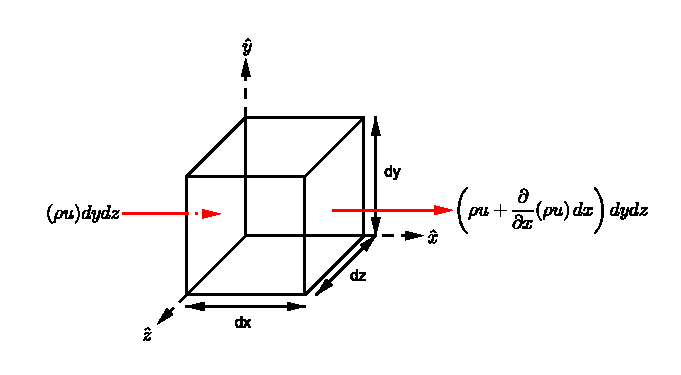
\includegraphics[scale=1]{images/massflowcube.eps}
\caption{\label{fig:massflowcube} Infinitesimal kontrollvolym för derivering av bevaranderelationer, här med massflödet exemplifierat}
\end{figure}

Betrakta nu en infinitesimal kontrollvolym som den i figur \ref{fig:massflowcube}. Integralerna över V ersätts med den infinitesimala volymen $dxdydz$ och \eqref{eq:convection:masscon} reduceras till

\begin{equation}
\label{eq:convection:massconinf}
0 = \left( \frac{\partial \rho}{\partial t} + \nabla \cdot \rho \mathbf{v}\right) dxdydz
\end{equation}

vilket, om $dxdydz$ förkortas bort, kan förenklas som

\begin{equation}
\label{eq:convection:continuity}
\boxed{ \; \; \;
0 = \frac{\partial \rho}{\partial t} + \nabla \cdot \left( \rho \mathbf{v} \right) 
\; \; \; }
\end{equation}

Om inkompressibilitet antas ($\rho$ = konstant) reduceras denna ekvation ytterligare till

\begin{equation}
\label{eq:convection:continuityinc}
\nabla \cdot \mathbf{v} = 0
\end{equation}

Detta är kontinuitetsekvationen för inkompressibla fluider.

Betrakta åter \eqref{eq:convection:reynolds} och sätt nu $B = m\mathbf{v}$. På samma vis som kontinuitetsekvationen \eqref{eq:convection:continuityinc} härleddes, fås för det infinitesimala volymelementet i figur sambandet

\begin{eqnarray}
\label{eq:convection:linear}
\sum \mathbf{F} & = & \frac{\partial}{\partial t} \left( \int_V \rho\mathbf{v} dV \right) + \int_{\partial V} \mathbf{v}\rho\left( \mathbf{v} \cdot \mathbf{n}\right)dV \nonumber \\
& = &\left(\frac{\partial}{\partial t} \left( \rho\mathbf{v} \right) + \nabla \cdot \left( \mathbf{v} \rho \mathbf{v}\right)\right)dxdydz \nonumber\\
& = &\left( \frac{\partial}{\partial t} \left( \rho\mathbf{v} \right) + \mathbf{v}\left(\nabla\cdot\rho\mathbf{v}\right) + \left(\rho\mathbf{v} \cdot \nabla\right) \mathbf{v}\right) dxdydz
\end{eqnarray}

ty enligt Newtons andra lag är tidsderivatan av rörelsemängden $m\mathbf{v}$ lika med summan av alla krafter som verkar på kroppen. $\dot{m}_i$ betecknar här massflödet $\rho\mathbf{v}_i\cdot\mathbf{A}_i$.

Det sista högerledet kan skrivas om som

\begin{equation}
\left( \mathbf{v}\left[ \frac{\partial \rho}{\partial t} + \nabla\cdot \rho \mathbf{v}\right] + \rho\left[ \frac{\partial \mathbf{v}}{\partial t} + u\frac{\partial\mathbf{v}}{\partial x} + v\frac{\partial\mathbf{v}}{\partial y} + w\frac{\partial\mathbf{v}}{\partial z} \right]\right)dxdydz.
\end{equation}

Första termen inom hakparentes är kontinuitetsekvationen \eqref{eq:convection:continuity} och går alltså bort.

Därmed reduceras \eqref{eq:convection:linear} till

\begin{equation}
\label{eq:convection:linearfinal}
\sum \mathbf{F} = \rho \left( \frac{\partial \mathbf{v}}{\partial t} + \mathbf{v}\cdot \nabla\mathbf{v} \right)dxdydz.
\end{equation}

Summan av de på volymen verkande krafterna måste nu utvecklas. Dessa krafter uppstår på grund av gravitation, tryck och viskositet. Andra krafter, såsom från elektromagnetiska fält, kan i sammanhanget anses vara försumbara. Gravitationskraften $\mathbf{F}_g$ beskrivs för den infinitesimala volymen med $\rho \mathbf{g} dxdydz = \rho g dxdydz \hat{z}$. Tryckkraften $\mathbf{F}_p$, i sin tur, ges av tryckgradienten $-\nabla \left( p \right) dxdydz$. Viskösa kraften $\mathbf{F}_{visc}$ är lite besvärligare att sammanställa. Anta att volymen är en Newtonsk fluid, det vill säga stresstensorn $\tau$ är linjärt proportionell mot hastighetsgradienten $\nabla\mathbf{v}$ med proportionaltitetskonstanten $\mu$, $\tau = \mu \nabla \mathbf{v}$. Den viskösa kraften verkande på kroppen blir då $\mathbf{F}_{visc} = \mu\Delta\mathbf{v}dxdydz$.

% Skriv om till integralrelationer och använd gauss sats, därefter infinitesimal volym

Vi har alltså ekvationssystemet

\begin{equation}
\label{eq:convection:momentum}
\addtolength{\fboxsep}{10pt} 
\boxed{ 
\begin{split} 
\rho\left(\frac{\partial u}{\partial t} + \mathbf{v}\cdot \nabla u\right) & = -\frac{\partial p}{\partial x} + \mu\Delta u\\
\rho\left(\frac{\partial v}{\partial t} + \mathbf{v}\cdot \nabla v\right) & = -\frac{\partial p}{\partial y} + \mu\Delta v\\
\rho\left(\frac{\partial w}{\partial t} + \mathbf{v}\cdot \nabla w\right) & = -\rho g -\frac{\partial p}{\partial z} + \mu\Delta w  
\end{split} 
} 
\end{equation}

% Energirelationen

Slutligen sätts i \ref{eq:convection:reynolds} $B=E$ för att söka ett uttryck för energins bevarande. Med antagandet att volymen inte utför något arbete blir $E = Q$, där $Q$ betecknar värmeenergin, och på samma vis som i avsnitt\ref{sec:heatconduction} blir $Q = c_p \rho dT$, vilket ger följande:

\begin{eqnarray}
\label{reynoldsenergyone}
\frac{dQ}{dt} & = & \frac{\partial}{\partial t} \int_V \frac{dQ}{dm}\rho dV + \int_{\partial V}\frac{dQ}{dm}\rho \mathbf{v} \cdot \mathbf{n} dA \nonumber\\
& = & \frac{\partial}{\partial t} \int_V c_p T \rho dV + \int_{\partial V} c_p T \rho \mathbf{v} \cdot \mathbf{n} dA \nonumber\\
& = & \left(\frac{\partial}{\partial t} \left( c_p T \rho \right) + \nabla\cdot c_p T \rho \mathbf{v}\right) dxdydz \nonumber\\
& = & c_p \rho \left( \frac{\partial T}{\partial t} + \mathbf{v}\cdot \nabla T\right)
\end{eqnarray}

Sista steget följer av att kontinuitetsekvationen bryts ut som i fallet med rörelsemängdsekvationen. För att utveckla vänsterledet betraktas återigen en infinetisemal volym såsom i figur \ref{fig:massflowcube}. Värmeenergiflödet in i volymen i x-led ges av $q_x dy dz$ medan utflödet ges av $\left[ q_x + \frac{\partial}{\partial x} \left( q_x\right)dx\right]dydz$ och analogt för y- respektive z-led. Totala ökningen av värmeenergi i kuben ges alltså av utflödet subtraherat från inflödet, vilket innebär att

\begin{equation}
\frac{dQ}{dt} = - \nabla \cdot \mathbf{q} dxdydz.
\end{equation}

$\mathbf{q}$ fås från Fouriers värmelag (se avsnitt \ref{sec:heatconduction}) vilket ger att

\begin{equation}
\label{reynoldsenergytwo}
\frac{dQ}{dt} = \left( - \nabla \cdot \left( -k \nabla T \right) \right)dxdydz
\end{equation}

och detta i sin tur leder till resultatet

\begin{equation}
\label{eq:convection:energy}\boxed{ \; \; \;
\nabla \cdot \left( k \nabla T \right) = c_p \rho \left( \frac{\partial T}{\partial t} + \mathbf{v}\cdot \nabla T\right)
\; \; \;}
\end{equation}

För homogena inkompressibla fluider i två dimensioner gäller alltså ekvationerna
\eqref{eq:convection:continuityinc}, \eqref{eq:convection:momentum} samt \eqref{eq:convection:energy}.

\subsection{Vindens konvektionskoefficient}

Då vinden blåser kommer en del värmeenergi överföras via konvektion, men istället för att lösa den invecklade konvektions-diffussionsekvationen används ofta något som kallas för vindens konvektionskoefficient, betecknat med $h$. I analogi med Fouriers värmelag, ekvation \ref{eq:conduction:fourier}, skrivs

\begin{equation}\boxed{ \; \; \;
q = hdT = h\left( T_{wall} - T_{\infty}\right).
\; \; \;}\end{equation}

där h alltså ka jämföras med det ovan härledda U-värdet. 

Denna konvektionskoefficient beskrivs ofta av en ekvation anpassad till empiriska resultat, och ett stort antal experiment har genomförts för att bestämma parametern, även om en helhetsbild saknas i dagsläget.

Vid fri (naturlig) konvektion, det vill säga då vinden är försumbar och luftcirkulationen följer av stigande varm luft, brukar h fås till mellan 2 och $\unit{25}{Wm^{-2}K^{-2}}$. Vid forcerad konduktion, det vill säga då vinden inte är försumbar, kan h variera från 25 till $\unit{250}{Wm^{-2}K^{-2}}$. \cite{ASHRAE09}

Traditionellt används ofta något som kallas för Nusselt-Jürges korrelation vid beräkning av konvektionskoefficienten, som lyder

\begin{equation}
h = 5.678 \left( a + b \left( \frac{965.42}{T_{out}}\left(|\mathbf{v}_{wind}\times \mathbf{n}|\right) \right)^c \right)
\end{equation}

där $\mathbf{n}$ betecknar väggens normalvektor, och a, b samt c beror på väggens ytegenskaper. För en skrovlig yta med $|\mathbf{v}_{vind}\times \mathbf{n}| < \unit{4.88}{ms^{-1}}$ fås att $a=1.09$, $b=0.23$ samt $c=1$, medan starkare vind ger $a=0$, $b=0.53$ samt $c=0.78$.

En mängd andra samband mellan konvektionskoefficienten och vindhastigheten har härletts, både teoritiskt och empiriskt, på grund av dess starka beroende av byggnadens ytegenskaper och area, men av anledningar som diskuteras i avsnitt \ref{sec:errors}.\cite{palyvos08}

% Skapa graf över T och v beroende

\subsection{Boussinesq approximation}

För flytkraftsdrivet flöde kan det vara lämpligt att använda sig av
Boussinesq approximation. Denna säger att det enda som påverkar trycket är
tyngdaccelerationen. Genom detta är det möjligt att sätta upp uttryck för densiteten
och tryckderivatorna enligt ekvationerna \eqref{eq:convection:density}
och \eqref{eq:convection:pressurez}. Här är
$\beta$ den volymetriska expansionskonstanten och
$T_0$ temperaturen som råder vid referensdensiteten $\rho_0$.

\begin{equation}
\label{eq:convection:density}
\rho = \rho_0[1-\beta(T-T_0)]
\end{equation}

\begin{equation}
\label{eq:convection:pressurez}
\frac{\partial p}{\partial z} = -\rho_0g
\end{equation}



\subsection{Finita element av inkompressibel fluid}

För att lösa Navier-Stokes ekvationer kan lämpligen en datormodell användas.
Här består denna modell av ett system uppsatt med Galerkins metod.
I denna lösning så begränsar vi dock oss till att enbart behandla statiska flöden
vilket genomförs genom att sätta alla tidsderivator till noll.

För att hantera trycket i \eqref{eq:convection:continuity}-\eqref{eq:convection:energy} används den tidigare nämnda Boussinesq approximation
samt penalty metoden för att göra hastighetsvektorn källfri och uppfylla
kontinuitetsekvationen. Det finns således inget direkt behov av att räkna ut trycket.
Vid användning av många sorters elementtyper som inte uppfyller Babuska-Brezzikriteriet
är detta dessutom nödvändigt då det annars kan bildas oönskade trycknoder. 
En annan möjlighet är att välja divergensfria element. \cite{babuska1973}\cite{segal2011}

Genom penaltymetoden beskrives här trycket som $p$ enligt ekvation
\eqref{eq:femconvection:penalty}. Här är $p_s$ någon form av idealt statiskt
tryck som är önskat. Detta tryck följer Boussinesq approximation. Med dessa
idealiseringar kan differentialekvationerna sättas upp igen. \cite{heinrich88}\cite{taylor79}
Som kan ses så leder den godtyckliga penaltyparametern $\lambda$ till att justera trycket
om hastighetsfältets divergens ej är identiskt noll. I viss litteratur anges 
det att penaltyparametern skall vara i storleksordningen $10^7$ men att den
är väldigt applikationsberoende. En för liten vald penaltyparameter leder till att
trycket inte elimineras. Andra problem uppstår vid en för stor parameter. Ekvationssystemet
kan bli svårlöst och få stabilitetsproblem när parametern blir
för stor i jämförelse med de andra delarna i differentialekvationen.\cite{reddy93}\cite{roy05}\cite{basak04}\cite{segal2011}

\begin{equation}
\label{eq:femconvection:penalty}
p = p_s - \lambda\nabla\cdot\mathbf{v}
\end{equation}

\noindent
Fortsatt skall trycket deriveras med avseende på de rumsliga variablerna vilket möjliggör
att eliminera trycket från differentialekvationerna. Dessa deriveringar kan ses i ekvation
\eqref{eq:femconvection:partx} samt \eqref{eq:femconvection:partz}. Notera att det statiska trycket
$p_s$ ej beror på $x$ vilket resulterar i att derivatan är noll.

\begin{equation}
\label{eq:femconvection:partx}
\frac{\partial p}{\partial x} = \frac{\partial p_s}{\partial x} -
\frac{\partial}{\partial x} \lambda\nabla\cdot\mathbf{v} = -
\frac{\partial}{\partial x} \lambda\nabla\cdot\mathbf{v}
\end{equation}

\begin{equation}
\label{eq:femconvection:partz}
\frac{\partial p}{\partial z} = \frac{\partial p_s}{\partial z} -
\frac{\partial}{\partial z} \lambda\nabla\cdot\mathbf{v} =
-g\rho_0 - \frac{\partial}{\partial z} \lambda\nabla\cdot\mathbf{v}
\end{equation}

\noindent
Detta förs in i momentekvationerna vilket ger ekvationerna \eqref{eq:femconvection:u} -
\eqref{eq:femconvection:T}. Här är det ekvationssystem som syftar att lösas.

\begin{equation}
\label{eq:femconvection:u}
\mathbf{v}\cdot\nabla u =
\frac{\lambda}{\rho_0}\nabla\cdot\mathbf{v} +
\nu\Delta u
\end{equation}

\begin{equation}
\label{eq:femconvection:w}
\mathbf{v}\cdot\nabla w =
\frac{\lambda}{\rho_0}\nabla\cdot\mathbf{v} + \nu\Delta w +g\beta(T-T_0)
\end{equation}

\begin{equation}
\label{eq:femconvection:T}
\mathbf{v}\cdot\nabla T = \alpha\Delta T
\end{equation}

\subsubsection{Svag formulering}

En finita elementlösning med Galerkins metod kräver att problemet reduceras till
ett ekvivalent variationsproblem. Här söks $T\in\Phi$, $u\in\Phi$ och
$w\in\Phi$ som uppfyller ekvation \eqref{eq:femconvection:variation}. Här
betecknar brackets skalärprodukt, $\mathbf{L}$ är differentialoperatorn
som betecknar systemet av differentialekvationer som $\mathbf{L}(T,u,w) = 0$.
$\Phi$ är rummet av alla testfunktioner $\phi$ som är kontinuerliga i
definitionsmängden $\Omega$ samt vars derivator är bitvis kontinuerliga på randen
$/Gamma$. De måste även vara $L^2$ integrabla.

\begin{equation*}
\label{eq:femconvection:variation}
\langle \mathbf{L}(T,u,w), \phi \rangle = 0\mbox{,  } \forall \phi \in \Phi
\end{equation*}


\section{Optimering med Newton-Raphsons metod}

När ett ekvationssystem är ickelinjärt kan ej exakta metoder som Gausseliminering användas
för ekvationslösning. Detta stötte vi till exempel på vid finita elementlösningen
av Navier-Stokes ekvationer i avsnitt \ref{sec:femconvection}.
I dessa fall måste approximativa optimeringsmetoder utnyttjas. En sådan
metod är Newton-Raphsons metod. Denna bygger på trunkerad Taylorutveckling 
av en funktion för att linjarisera ett ickelinjärt ekvationssystem
$\mathbf{f}(\mathbf{x}) = 0$
vilket kan ses i ekvation \eqref{eq:newtonsmethod:taylor}. Här är
$\mathbf{J}_f(\mathbf{x})$ jacobianen för $\mathbf{f}(\mathbf{x})$. 

\begin{equation}
\label{eq:newtonsmethod:taylor}
\mathbf{f}(\mathbf{x} + \Delta\mathbf{x}) \approx \mathbf{f}(\mathbf{x}) +
\mathbf{J}_f(\mathbf{x})\Delta\mathbf{x}
\end{equation}

\noindent
Principen går ut på att algoritmen upprepat gissar nya lösningar där de
nya lösningarna följer den negativa jacobianen. Till en början är en god initial gissning
$\mathbf{x}_0$ ett kriterie för att Newton-Raphson skall konvergera. Därefter så beräknas
funktionsvärdet $\mathbf{f}(\mathbf{x}_0)$ samt jacobianen $\mathbf{J}_f(\mathbf{x}_0)$.
Dessa används för att beräkna nästa gissning genom att lösa
\eqref{eq:newtonsmethod:guess} och beräkna nästa $\mathbf{x}$ med
\eqref{eq:newtonsmethod:nextx}. \cite{heath2002}

\begin{equation}
\label{eq:newtonsmethod:guess}
\mathbf{J}_f(\mathbf{x}_n)\Delta\mathbf{x}_n = -\mathbf{f}(\mathbf{x_n})
\end{equation}

\begin{equation}
\label{eq:newtonsmethod:nextx}
\mathbf{x}_{n+1} = \mathbf{x}_n + \Delta\mathbf{x}_n
\end{equation}

\noindent
Itereringen bör avbrytas då ett maxantal itereringar har uppnåtts och funktionen
ej har konvergerat alternativt när felet är tillräckligt litet. En av styrkorna 
med denna algoritm är dess kvadratiska konvergens mot enkelrötter. \cite{ympa95}
En svaghet med Newton-Raphson är att det i många fall ej är möjligt att analytiskt beräkna
jacobianen. Istället måste andra algoritmer untnyttjas som till exempel finita differensmetoden
för beräkning av jacobianen. Omvägar som denna bidrar till att lösningsprocessen blir mycket
mer omständig och processorintensiv. 

\subsection{Konvergens samt konvergenskriterier}

För att enklare förstå några problem som kan uppstå med Newton-Raphsons metod kan det vara lämpligt
att repetera beviset av dess kvadratiska konvergens. Definiera en funktion $f(x)$ enligt \eqref{eq:newtonproof}.
Antag att den roten $f(x) = 0$ existerar för $x = \alpha$.

\begin{align}
f: & \mathbb{R} \to \mathbb{R} \nonumber \\
   & x \mapsto f(x) \label{eq:newtonproof}
\end{align}

\noindent
Härnäst genomförs en taylorutveckling av funktionen $f(x)$ i ekvation \eqref{eq:newtonprooftaylor}.
Den kvadratiska termen är här Lagranges restterm med parametern $\xi_n \in [\alpha, x_n]$.

\begin{equation}
\label{eq:newtonprooftaylor}
f(\alpha) = f(x_n) + f^\prime(x_n)(x_n-\alpha) + \frac{f^{\prime\prime}(\xi_n)}{2}(x_n-\alpha)^2
\end{equation}

\noindent
Nu kan förstaderivatan av $f(x_n)$ divideras över samt $f(\alpha)$ är känt att vara noll.
Efter detta identifieras $f(x_n)/f^\prime(x_n) = x_n-x_{n+1}$ och ersätts. Slutligen så ses
det i ekvation \eqref{eq:newtonqed} att $x_{n+1}-\alpha \propto (x_{n}-\alpha)^2$.

\begin{equation}
0 = \frac{f(x_n)}{f^\prime(x_n)} + \alpha - x_n + \frac{f^{\prime\prime}(\xi_n)}{2f^\prime(x_n)}(x_n-\alpha)^2
\Rightarrow
\end{equation}

\begin{equation}
\label{eq:newtonqed}
x_{n-1} - \alpha = - \frac{f^{\prime\prime}(\xi_n)}{2f^\prime(x_n)}(x_n-\alpha)^2 
\end{equation}

\noindent
För att ovanstående bevis ska gälla så måste andraderivatan vara uppåt begränsad, förstaderivatan får ej
vara noll och den högre ordningens derivator får ej vara av stor betydelse för funktionens uppträdande
nära roten $f(x) = 0$. Rent praktiskt innebär detta att en god gissning är essentiell för att få
konvergens i metoden. Även med en god gissning så kan problem uppstå om derivatan av funktionen
förändras snabbt i omgivningen av $x$. Detta kan resultera i både att nästa gissning ligger för långt
bort och för nära. Det förstnämnda problemet innebär att metoden hoppar över roten vilket till och med
kan innebära att metoden divergerar. Det andra problemet är mindre allvarligt då det endast innebär 
att metoden förlorar sin kvadratiska konvergens.

\subsection{Förbättrad Newton-Raphson}

En metod för att hantera att metoden hoppar över rötter är att i varje steg försöka minimera $|f(x_{n+1})|$.
Rent praktiskt innbär detta att vi väljer en konstant $0 \le k_n \le 1$ och genomför ett modifierat
Newtonsteg enligt ekvation \eqref{eq:newtonmodified}.

\begin{equation}
\label{eq:newtonmodified}
x_{n+1} = x_n - k_n\frac{f(x_n)}{f^\prime(x_n)}
\end{equation}

\noindent
För att identifiera det optimala valet av $k_n$ kan godtycklig linjesökningsalgoritm användas. Ett val av metod
är att behandla det analytiskt för att göra metoden mindre processorintensiv. En ny funktion definieras
enligt ekvation \eqref{eq:newtong} med $\Delta x_n = f(x_n)/f^\prime(x_n)$.

\begin{equation}
\label{eq:newtong}
g(k_n) = f(x_n- k_n\Delta x_n)
\end{equation}

\noindent
I ekvation \eqref{eq:newtongmin} deriveras funktionen med avseende på $k_n$ i punkten $k_n=0$
och kedjeregeln används för att skriva om uttrycket till något som är användbart.

\begin{align}
\frac{\partial g(k_n)}{\partial k_n}\,\bigg|_{k_n=0} & = 
\left(\frac{\partial g(k_n)}{\partial (k_n\Delta x_n)}
\frac{\partial k_n \Delta x_n}{\partial k_n}\right)\,\bigg|_{k_n=0} = \nonumber \\
x_n \frac{\partial f(x_n- k_n\Delta x_n)}{\partial (k_n\Delta x_n)}\,\bigg|_{k_n=0} & = 
-\Delta x_n f^\prime(x_n) = - f(x_n)
\label{eq:newtongmin}
\end{align}

\noindent
Ett förslag på algoritm är nu att i varje iterationssteg först beräkna det fulla newtonsteget motsvarande $k_n=1$.
Är då $f(x_{n+1}) < f(x_n)$ så kan steget godtagas. Stämmer inte detta så beräkas derivatan av $g(k_n)$ och
funktionen $g(k_n)$ ansätts vara ett polynom av andra ordningen enligt ekvation \eqref{eq:newtonfit}.

\begin{equation}
\label{eq:newtonfit}
g(k_n) = ak^2_n + bk_n + c
\end{equation}

\noindent
Nu kan de kända värdena $g(0)$, $g(1)$ samt $g^\prime(0)$ användas för att lösa ut koefficienterna i polynomet.
Dessa kan slutligen användas för att beräkna derivatan av $g(k_n)$ för att hitta dess minimum och således
hitta den optimala parametern $k_n$.

\noindent
Om denna metod skall användas för att lösa ett ekvationssystem istället för en realvärd funktion i en dimension
så behövs något mått sättas upp. Problemet som önskas att lösas är $\mathbf{F}(\mathbf{x}) = 0$.
Funktionen som skall minimeras kan då med fördel väljas till $f(\mathbf{x}) = \mathbf{F}(\mathbf{x})^2/2$.
På ett analogt sätt ovan så beräknas derivatan av funktionen $g(k)$ till ekvation \eqref{eq:newtonvecg}.\cite{fortran77}

\begin{equation}
\label{eq:newtonvecg}
g_n^\prime(0) = - \mathbf{F}(\mathbf{x_n})^2 \le 0
\end{equation}

\noindent
För att hitta roten $\mathbf{F}(\mathbf{x}) = 0$ så ansätts som ovan ett polynom där koefficienterna beräknas.
Som kan ses så existerar det ett $k_n$ så att $\mathbf{F}(\mathbf{x}_{n+1}) \le \mathbf{F}(\mathbf{x}_n)$ ty
$g^\prime(0) \le 0$ och enbart noll om roten redan är funnen.


\section{Konstanta energiflöden}

En del av energiflödena är relativt konstanta sett till en längre tidsperiod. Dessa är främst värme från elektriska apparater, så som kylskåp och datorer, människors kroppsvärme och varmvattencirkulation. Även kylningen från husets grund anses vara konstant.

Väldigt liten del av den energi som förbrukas i en elektrisk apparat blir till något annat än värme. Därför låter vi det energiflödet motsvaras av fastighetens energiförbrukning. Den kan läsas av kontinuerligt och på så sätt reglera aktivt tillförd energi\footnote{Aktivt tillförd energi: Den energitillförsel som kan regleras och tillförs via radiatorerna.}.

Människornas utstrålade kroppsvärme kan beräknas genom att de antas vara svartkroppar. Stefan-Boltzmanns lag säger då att utstrålade energi per yt- och tidsenhet är $j=\sigma T^4$, där $T$ är temperaturen och $\sigma=\unit[5.6705\cdot 10^8]{Wm^{-2}K^{-4}}$ \cite{physicshandbook}. På samma sätt beräknas den energi som strålas in mot kroppen från omgivningen. Nettostrålningen från en människa kan då ses i ekvation \eqref{eq:constantsources:stefan} där $T_k=37^{\circ}C=310K$ är kroppstemperaturen och $T_r=20^{\circ}C=293K$ är rumstemperaturen. Multiplicerat med en människas area, ungefär $\unit[2]{m^2}$, fås en nettoeffekt på $\unit[211]{W}$. I själva verket reduceras denna effekt av en rad faktorer. Exempelvis är hudens temperatur lägre än kroppstemperaturen samtidigt som klädesplagg reducerar effektutstrålningen något. Det är allmänt vedertaget att man kan sätta nettoeffekten till ungefär $\unit[50-100]{W}$.

\begin{equation}
\label{eq:constantsources:stefan}
j=\sigma \left( T_k^4 - T_r^4 \right)
\end{equation}
\noindent
I huset cirkulerar hela tiden varmvattnet för att alltid kunna tillgodose de boendes behov av varmvatten utan dröjsmål. Efter en tur i systemet sjunker temperaturen på varmvattenet med tre grader. Detta motsvarar en energitillförsel till fastigheten på \textcolor{red}{??} $\unit[]{W}$.

Grunden huset står på har en randtemperatur på ungefär $6^{\circ}\mbox{C}$ från marken. Den kan antas vara konstant då huset grund ligger en bit ned under marken. Enligt SLU, Sveriges Lantbruksuniversitet, kan marktemperaturen antas vara konstant från $\unit[1,6]{m}$ under markytan \cite{SLU}. Deras data kommer från Uppsala vilket borde vara jämförbart med Göteborg. Huset står på en grund som består av ett luftgap och sedan $\unit[0,25]{m}$ betong. Längst ned i huset finns en källare som är ouppvärmd \textcolor{red}{??}. Det energiläckage som då blir genom husets grund ned i marken kan beräknas uppgå till \textcolor{red}{??} $\unit[]{W}$.

\section{Strålning genom glas}
\label{sec:sunthroughwindows}
Solstrålning genom fönster orsakar snabba temperaturökningar i inomhusklimatet. Hur snabba och stora dessa temperaturökningar blir beror på en mängd parametrar varav de viktigaste omfattas av fönstrets utformning, det vill säga glasets reflektivitet och emmissitivitet, strålningens infallsvinkel som beror av tid på dagen och året och ytorna inomhus som solstrålningen faller på, så som persienner, gardiner, vägger och möbler. Fönstrets reflexivitet och emmisivitet är beror av solens infallsvinkel.

%\begin{itemize}
%\item{
%fönstrets utformning, det vill säga glasets reflektivitet och emmissitivitet.
%}
%\item{
%vinkeln relativt fönstret som strålningen infaller vid, det vill säga tid på dagen och året. Detta är starkt förknippat med föregående punkt. 
%}
%\item{
%de inomhus belägna ytorna som solstrålningen faller på, det vill säga persienner, gardiner, väggar, möbler, etcetera.
%}
%\end{itemize} 

\subsection{g-värden}\label{gvalue}

För att ange transmittansen av solstrålning genom fönster brukar man använda vad som kallas för g-värden (ibland även kallat ''Solar Factor''). Detta värde, mellan noll och ett, anger hur mycket av infallande solstrålnings normalprojektion som släpps igenom. Men eftersom ett sådant värde också beror på strålningens infallsvinkel (på grund av ökande reflektion med ökande vinkel) är den ofta svår att beräkna.

Enligt \cite{karlssonroos99} förändras detta vinkelberoende främst med antalet glas (flerglasfönster) samt typ av eventuella beläggningar på glaset. I samma artikel visades också att g-värdenas vinkelberoende kan approximeras med ett polynom

\begin{equation}\label{eq:radiationwindowstheory:gvalue}
g = g_0 \left( 1 - az^{\alpha} - bz^{\beta} - cz^{\gamma} \right)
\end{equation}

där $g_0$ är g-värdet då strålningen infaller vinkelrätt mot ytan, $a+b+c=1$ och $z=\theta/90$ då $\theta$ är vinkeln, mätt i grader, mellan fönstrets normal och solstrålningens riktning. Koefficienterna och exponenterna i \eqref{eq:radiationwindowstheory:gvalue} beror på typen av fönster, och i \cite{karlssonroos99} har empiriska undersökningar lett till aproximationen

\begin{align}\label{eq:gconstants}
a & = 8, & b & = 0.25/q, & c & = (1-a-b) \nonumber \\
\alpha & = 5.2 + 0.7q, & \beta & = 2, & \gamma & = (5.26+0.06p) + (0.73+0.04p)q
\end{align}

där p är antalet rutor i fönstret (treglasfönster medför $p = 3$) och q är en parameter, $1 \le q \le 10$, som varierar beroende på beläggningar på glasets yta. Exempelvis har ett treglasfönster utan beläggningar värdet $q=4$.

Det beräknade g-värdet kan sedan användas för att uppskatta energiflödet genom fönstret. Anta att en pyranometer anger solstrålningsintensiteten $I_0$ i $\unit{W m^{-2}}$. Då ges det totala energiflödet $Q$ av sambandet 

\begin{equation}\label{eq:totalsun}
Q = g \left( \theta \right)\cdot A \cdot I_0 \cos{\theta} \unit[]{W},
\end{equation}

där $A$ är fönstrets area och $\theta$ är vinkeln solen bildar mot ytans normal.

\subsection{Långvågsstrålning}

När ytorna inne i byggnaden är varmare än ytorna utomhus resulterar detta i ett utflöde av långvågig strålning vars storlek kan approximeras med Stefan-Boltzmanns lag, \ref{eq:boltzmanslag}. Antag att interiören håller en konstant temperatur på $T_{in} = \unit[20]{^{\circ}C}$ och att de för interiören genom fönstrena synliga utomhusytorna håller en konstant temperatur på $T_{out} = \unit[6]{^{\circ}C}$. Detta leder till ett flöde $j^{\star} = \sigma \left( T_{in}^{4}-T_{out}^4\right) = \sigma \left( 293^4-279^4 \right) \approx \unit[74]{Wm^{2}}$. Genom ett fönster fås då utstrålningen $Q_{IR}=A\cdot\unit[74]{W}$, där $A$ är fönstrets area. Vidare måste hänsyn tas till att glasrutorna reflekterar en andel av långvågsstrålningen. För en ensam glasruta utan beläggningar gäller då att en normal fönsterruta reflekterar i grova drag $10\%$ av den utgående strålningen \cite{gelin05}.

\begin{figure}[hpbt]
\centering

\includegraphics[scale=2]{images/tripleglazing.eps}
\caption{Visualisering av variabelnamnen använda vid härledning av reflektionsparametern för treglasfönster.}
\label{fig:tripleglazing}
\end{figure}

För en treglasruta gäller en något mer komplicerad annan reflektionsparameter. Betrakta figur \ref{fig:tripleglazing}. För $I_1$, den intensitet som släpps igenom första rutan, gäller att 

\begin{equation}
I_1=I_{in}\left( 1-a \right).
\end{equation}

På grund av en oändlig följd av reflektioner, även från den del av $I_3$ som passerar ruta 2 igen, blir $I_2 = \left( 1-a \right) I_1 \sum_{n=0}^{\infty} a^{2n} + a \left( 1-a \right)^2 I_3 \sum_{n=0}^{\infty} a^{2n}$. Men samtidigt måste också $I_3 = aI_2\sum_{n=0}^{\infty} a^{2n}$ vilket, om $I_2$ bryts ut, ger att

\begin{equation}
I_2 = \frac{\left( 1-a \right) I_1 \sum_{n=0}^{\infty} a^{2n}}{1-\left( 1-a \right)^2a^2\left(\sum_{n=0}^{\infty} a^{2n}\right)^2}.
\end{equation}

Detta tillsammans med det faktum att 

\begin{equation}
I_{ut} = \left( 1-a \right)I_2\sum_{n=0}^{\infty} a^{2n}
\end{equation}

ger, då dessa tre samband kombineras, att

\begin{equation}
I_{ut} = \frac{\left( 1-a \right)^3\left( \sum_{n=0}^{\infty} a^{2n}\right)^2}{1-\left( 1-a \right)^2a^2\left(\sum_{n=0}^{\infty} a^{2n}\right)^2}I_{in}.
\end{equation}

Notera nu att $\sum_{n=0}^{\infty} a^{2n} = \frac{1}{1-a^2}$ på grund av geometriska seriers egenskaper. Sätt in detta och förenkla så fås tillslut att

\begin{equation}
I_{ut} = \frac{\left( 1-a \right)^3}{\left(\left( 1-a^2\right)^2 - \left(1-a\right)^2 a^2\right)}I_{in} = 0,75 \cdot I_{in}
\end{equation}

då $a=0.1$.

\subsection{Johanneberg 7:8 – en beskrivning av fastigheten på Walleniusgatan}

\subsubsection{Huset som bostad}
% Det är så här stort och har så här många rum, så här högt i tak o.s.v. 

% De olika gränsytornas material och uppbyggnad.
\subsubsection{Väggarna}

\subsubsection{Taket}

\subsubsection{Grunden}


\subsubsection{Huset byggandstil och histora}
% Hur tänkte de när de byggde och renoverade huset?
% Vad ville de uppnå och vilka regler och normer hade man att hålla sig till?

\subsubsection{Byggnadsfysikens betydelse}
% Att huset är byggt så här vad betyder det för hur huset påverkas och hur huset är att bo i?

\subsubsection{Uppvärmning}
% Kortfattat vad finns det för värmeförsörjningssystem idag?
% Hur fungerar det? Varför valde man det?

\subsubsection{Ventilation}
% Hur fungerar ventilationen?
\section{Definition av väder för tillämpningar i denna rapport}
\label{subsec_weather}
Vår uppdragsgivare vill undersöka hur inomhustemperaturen påverkas av vädret. Tesen är att man kan få en mer korrekt styrning av inomhustemperaturen om man inte bara låter den påverkas av utomhustemperaturen, utan även av fler väderparamterar. Han har därför installerat en väderstation, se avnitt~ \ref{subsec_weathertransmitter}.

Begreppet väders vardagliga användningsområde är mycket brett och behöver därför avgränsas för att definiera de väderparameterar som behandlas inom projektet.

Kortfattat definieras vädret som det väderstation tillsammans med solintensitetsmätaren mäter. Så som finns beskrivet i avsnitt~\ref{subsec_weathertransmitter} mäter vi vädret med utrustning som tar in vindens hastighet och riktning, lufttemperaturen, lufttryck, relativ fuktighet samt regn och hagels varaktighet och intensitet. Vi kommer dock att bortse helt ifrån hagel då detta sker så sällan och i så korta perioder att det kan antas försumbart.  Dessutom mäter solintensitetsmätaren solens intensitet och varaktighet, se avsnitt~\ref{subsec:sunmeter}. % Källa på hur ofta (sällan) det haglar i Sverige. 

Tanken är att man ska kunna beskriva allt väder som en temperatur, antingen som den utomhustemperatur man bör reglera efter eller som den inomhustemperatur huset skulle få med befintlig aktivitet men utan uppvärmning, alltså ett mått på hur många grader man måste värma. Dessa två mått kallas ekvivalent temperatur och free-running temperature vilka beskrivs i avsnitt~\ref{sec:ekv_temp} respektive avsnitt~\ref{sec:freerunningtemp}. 

Från studier med hjälp av beräkningstjänsten Wolfram Alpha\cite{wolframalpha} av hur luftfuktighet kan påverkar luftens värmeledningsförmåga, får vi att den har väldigt liten betydelse. Man kan se en liten skillnad vid mycket höga luftfuktigheter (upp emot 90 \%) vid de högre temperaturerna, över $\unit[25]{^\circ C}$. Detta torde vara försumbart eftersom skillnaden är liten och endast vid väderförhållanden som inträffar relativt sällan i vårt klimat.

Hur regn och fukt påverkar fastighetensklimat har inte behandlats inom det här projektet.
Det kan dock antas att en hel del energi försvinner när väggen blir blöt och vattnet avdunstar. Troligen kyler regnet även luften.

Ytterligare en parameter som inte behandlas till är snö. När snön har lagt sig på taket kan man anta att den har en isolerande effekt. Vi kan inte mäta om och i så fall hur mycket snö det ligger på taket. Enligt SMHI\cite{SMHIdata}
rör det sig enbart om 25-50 dygn med snö i Göteborg per år. Detta påverkar dessutom främst de översta lägenheterna, de på vinden. Har man däremot en enplansvilla i Norrland kan man anta att detta är en mer betydande parameter, men det är alltså inget vi kommer att undersöka.

\subsection{Väderstationen}
\label{subsec_weathertransmitter}
I rapporten låter vi de parametrar som väderstationen tar in definiera vädret, se avnitt~\ref{subsec_weather}. Väderstationen som vår uppdragsgivare installerat är en Vaisala Weather Transmitter WXT520. Den mäter sju olika värden: vindens hastighet och riktning, lufttemperaturen, lufttrycket, den relativa fuktigheten samt regn och hagels varaktighet och intensitet. I tabell \ref{tbl:weathertransmitter} beskrivs stationens mätområde, noggrannhet och upplösning för de olika parametrarna. Vi har således väldigt liten nytta av att låta våra beräkningar vara noggrannare än väderstationen kan mäta.

\begin{table}[htdp]
\caption{Tekniska data för väderstationen, \cite{datasheet_weathertransmitter}}

\begin{center}
\begin{tabular}{|l | l l l|}
\hline
\textbf{Väder} & \textbf{Mätområde} % range
 & \textbf{Noggrannhet} % accuracy
 & \textbf{Upplösning} \\ % resolution
\hline
\rule{0pt}{3ex}Vindhastighet & $0$ -- $\unit[60]{m~s^{-1}}$ & $\pm3$ -- $5\%$ & $\unit[0,1]{m~s^{-1}}$ \\ 
\rule{0pt}{3ex}Vindriktning & alla riktningar & $\pm 3^{\circ}$ & $1^{\circ}$ \\
\rule{0pt}{3ex}Temperatur & $-52$ -- $\unit[+60]{^{\circ}C}$ & & $\unit[0,1]{^{\circ}C}$ \\
\rule{0pt}{3ex}Lufttryck & $600$ -- $\unit[1100]{hPa}$ & $0,5$ -- $\unit[1]{hPa}$ & $\unit[0,1]{hPa}$ \\
\rule{0pt}{3ex}Luftfuktighet & $0$ -- $\unit[100]{\%RH}$ & $\pm3$ -- $\unit[ 5]{\%RH}$ & $\unit[0,1]{\%RH}$ \\
\rule{0pt}{3ex}Regn &  & $\unit[5]{\%}$ & \unit[0,01]{mm} \\
~varaktighet & & & $\unit[10]{s}$\\
~intensitet & $\unit[0\mhyphen 200]{mm~h^{-1}}$ & & $\unit[0,1]{mm~h^{-1}}$ \\
\rule{0pt}{3ex}Hagel &  &  & 0,1 $\unit{cm^2}$ \\
~varaktighet & & från första träffen & 10 s\\
~intensitet & & & 0,1 $\unit{cm^{-2}~h^{-1}}$\\
\hline
\end{tabular}
\end{center}
\label{tbl:weathertransmitter}
\end{table}

\subsection{Solintensitetsmätaren}\label{subsec:sunmeter}
Mätaren för solintensitet som finns monterad på fastigheten är en Pyranometer CMP3 av märket Kipp \& Zonen. Den mäter våglängder från $300$ till $\unit[2800]{nm}$, vilket täcker in större delen av den solstrålning som når jorden. Ur databladet fås också att osäkerhet för en dag kan väntas vara under $\unit[10]{\%}$. Den största möjliga instrålningen den klarar av att mäta är $\unit[2000]{W m^{-2}}$ vilket är väl över maximala möjliga värde på jorden om man enbart mäter strålning från solen. Den uppfyller gott och väl behoven för studien.\cite{datasheet_sun}




\section{Free-running temperature – en konceptuell beskrivning}
\label{sec:freerunningtemp}

Free-running temperature är ett begrepp som används för att sammanfatta olika 
värmeflödens påverkan på byggnader. Det finns tyvärr ingen bra svensk översättning 
men det kan beskrivas som den inomhustemperatur som fås om byggnaden används 
normalt men aktivt tillförda energin, det som normalt kallas uppvärmning via radiatorer, 
stängs av.

I en fastighet finns många olika värmekällor, så som värme från elektriska apparater, 
människorna som vistas där, belysning och varmvatten för hushållsbruk. All den värmen
 bidrar till att värma upp huset. På grund av termodynamikens huvudsatser vet vi att 
 kroppar i kontakt alltid strävar efter jämvikt och på så sätt får vi ytterligare energiflöden på 
 grund av vind, sol och utomhustemperatur.

Normalt används sedan den tillförda energin till att utjämna detta. Genom att inte värma 
fastigheten kan man istället räkna på hur mycket energi man behöver tillföra fastigheten 
vid olika tidpunkter för att nå önskad inomhustemperatur.

Denna storhet kan givetvis mätas, men eftersom man vill bibehålla aktiviteten är detta troligen inte så populärt hos de som använder byggnaden, speciellt inte med det klimat vi har i Sverige. Vi har istället valt att använda våra modeller för att beräkna den.

Måttet free-running temperature kan användas till flera olika saker. Det enklaste är att 
jämföra olika byggnader, där man i och med den fortsatt aktiviteten i byggnaden jämför
 dem med hänsyn till vad de används till – ett vilohem eller en idrottshall har troligen 
 ganska olika free-running temperature även om de skulle ha exakt samma 
 byggnadstekniska specifikation. Vid beräkning av värdet behöver man givetvis inte ta 
 hänsyn till detta men det kan ändå vara intressant för undersöka energibehovet.

Ett annat användningsområde är att sätta upp en statistisk modell där man kan visa hur 
energibehovet förändras beroende på verksamhet och väderparametrar. Detta ligger 
betydligt närmare till hands för det här arbetet och i förlängningen kanske det kan leda till 
en mer anpassat reglersystem för uppvärmningen av byggnaden.

<<<<<<< HEAD
\section{Ekvivalent temperatur}

Kort sagt är ekvivalent temperatur det värde man ersätter utomhustemperaturen för att ta 
hänsyn till fler väderparametrar än just utomhustemperaturen i styrningen av en 
klimatanläggning.

Att bara ta hänsyn till utomhustemperaturen vid injustering av klimatsystem är enkelt. 
Tyvärr är det lite för enkelt för att det ska bli riktigt bra, eftersom flera andra 
väderparametrar, främst sol och vind, värmer och kyler fastigheten i olika grad. I resultatdelen i den här rapporten visas det mer exakt hur mycket.

De energiflöden i väggen som orsakas av väderleken summeras med energiflödet 
som uppkommer av utomhustemperaturen. Dessa jämförs sedan med energiflöden från 
olika utomhustemperaturer, utan övrig väderpåverkan, och den temperatur som ger 
samma energiflöde kallas ekvivalent temperatur. Denna kan sedan ersätta 
utomhustemperaturen som indata till klimatsystemet och ge ett jämnare inomhusklimat.

% är det bra
% varför används det


% Tidigare text:
%Antag att det bara finns ett sorts väder, där temperaturen är den enda variabeln. Det
% skulle innebära att man kan hänföra hur mycket energi som går åt för att värma upp 
% någonting direkt till utetemperaturen. Det finns oändligt antal olika vädertyper, och fler 
% parametrar måste tas i beaktning då man räknar ut hur mycket energi som måste tillföras
%  huset. En ekvivalent temperatur för en viss vädertyp skulle således motsvara den 
%  temperaturen, i ett optimalt klimat, som kräver tillförsel av samma energimängd för att 
%  upprätthålla efterfrågat klimat.
=======
\section{Ekvivalent temperatur}

Kort sagt är ekvivalent temperatur det värde man ersätter utomhustemperaturen för att ta 
hänsyn till fler väderparametrar än just utomhustemperaturen i styrningen av en 
klimatanläggning.

Att bara ta hänsyn till utomhustemperaturen vid injustering av klimatsystem är enkelt. 
Tyvärr är det lite för enkelt för att det ska bli riktigt bra, eftersom flera andra 
väderparametrar, främst sol och vind, värmer och kyler fastigheten i olika grad. I resultatdelen i den här rapporten visas det mer exakt hur mycket.

De energiflöden i väggen som orsakas av väderleken summeras med energiflödet 
som uppkommer av utomhustemperaturen. Dessa jämförs sedan med energiflöden från 
olika utomhustemperaturer, utan övrig väderpåverkan, och den temperatur som ger 
samma energiflöde kallas ekvivalent temperatur. Denna kan sedan ersätta 
utomhustemperaturen som indata till klimatsystemet och ge ett jämnare inomhusklimat.

% är det bra
% varför används det


% Tidigare text:
%Antag att det bara finns ett sorts väder, där temperaturen är den enda variabeln. Det
% skulle innebära att man kan hänföra hur mycket energi som går åt för att värma upp 
% någonting direkt till utetemperaturen. Det finns oändligt antal olika vädertyper, och fler 
% parametrar måste tas i beaktning då man räknar ut hur mycket energi som måste tillföras
%  huset. En ekvivalent temperatur för en viss vädertyp skulle således motsvara den 
%  temperaturen, i ett optimalt klimat, som kräver tillförsel av samma energimängd för att 
%  upprätthålla efterfrågat klimat.
>>>>>>> 016a6be50697be1083f4accc334f848f4a268cd5


%Metod
\chapter{Metod}

I detta kapitel presenteras den metodik som tillämpats vid beräkning av olika energiflöden och bygger på det teoretiska underlag som presenterats i föregående kapitel. Byggnaden kommer här delas upp i de två beståndsdelarna grunden – som påverkas av vädret via med marken som värmebuffert – samt byggnadsskalet – med väggar, tak och fönster vars yta direkt påverkas av vädret. Dessutom tillkommer solinstrålningen genom fönster och ofrivillig ventilation på grund av vind, vilka betraktas helt fristående.

Vi börjar med att de analytiska beräkningar som beskriver solinstrålningen och går sedan direkt in på att beskriva hur ett statiskt värmeflöde genom en vägg kan beräknas. Vidare beskrivs hur finita elementmetoden har används för att behandla statiska flöden, som används här för att beräkna luftflödet längs väggen när det blåser.

Slutligen finns ett avsnitt som beskriver hur vi med hjälp av programmet Comsol beräknar påverkan på fastigheten från ofrivillig ventilation, det vill säga hur mycket energi som försvinner genom vind som penetrerar huset. 

\section{Strålning genom glas}\label{sec:sunthroughwindowsmethod}

I följande avsnitt presenteras de metoder som använts vid beräkning av energiflöde genom fönster i byggnaden. Vi börjar med att beskriva hur direkt solinstrålning genom fönster kan beräknas. Därefter följer ett kort stycke med redogörelser över hur vi går tillväga för att beräkna energiflödet via svartkroppsstrålning mellan rummet och omgivningen. Notera särskilt avsnitt \ref{subsec:otherradiation} som kortfattat beskriver ett par strålningssituationer som försummats. Avslutningsvis presenteras en metod som används för att uppskatta hur mycket energi man kan spara genom att ta hänsyn till den direkta solinstrålningen.

\subsection{Soltimmar under dygnet}
\label{subsec:sunhours}
Under året så varierar antalet soltimmar. Detta kommer av att jordens axel ej är paralell
med jordens rotationsaxel kring solen. I praktiken innebär detta att det är mindre soltimmar
under vinterhalvåret och fler under sommarhalvåret. Då jordens bana kring solen är nästan
cirkulär kan vi approximera antalet soltimmar per dygn som en trigonometrisk funktion.
För Göteborg approximerar vi att årets kortaste dag är $\unit[6]{ timmar}$ och $\unit[32]{minuter}$ och årets längsta
dag är $\unit[17]{ timmar}$ och $\unit[28]{ minuter}$. \cite{sunup} Sedan noterar vi att dagen är som kortast runt den $20$
december.
Detta tillåter oss då att teckna dygnets soltimmar $\tau$ som ekvation \eqref{eq:sunhours}. Här
är $t$ tiden i månader där $t=0$ motsvarar första januari och $t$ är periodiskt över $12$ månader.

\begin{equation}
\label{eq:sunhours}
\tau = 12 - \left(6-\frac{32}{60}\right)\cos\left[\frac{\pi}{6}\left(t+\frac{1}{3}\right)\right]
\end{equation}

\noindent
Fastigheten somdetta arbete undersökerhar en eldningsperiod som går från början av oktober
till slutet av april. Av denna anledning önskasdet attberäknahur många soltimmar detsnitt är per
dag. För detta syfte tecknas medelvärdet $\bar{\tau}$ enligt

\begin{equation}
\label{eq:taubar}
\bar{\tau}= \frac{ \int^{16}_9 \left(12 - \left[6-\frac{32}{60}\right]\cos\left[\frac{\pi}{6}\left(t+
\frac{1}{3}\right)\right]\right)\mathrm{d}t}{\int^{16}_9 \mathrm{dt}}
\end{equation}

\noindent
När \eqref{eq:sunhours}och \eqref{eq:taubar} evaluerades gavs 
resultatet som kan ses i figur \ref{fig:sunhours}.
Medelvärdet harhär beräknats vara $\bar{\tau}=\unit[9,39]{~timmar~per~dygn}$.
\begin{figure}
\centering
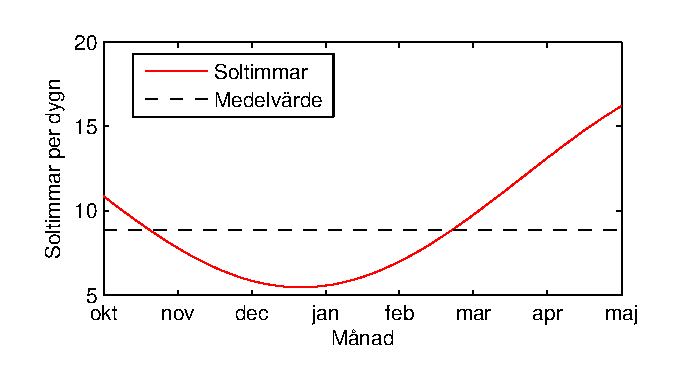
\includegraphics{images/sunhours.eps}
\caption{Antal timmar i ett dygn då solen är ovanför horisonten beräknat för månaderna under eldningsperioden.
Här är medelvärdet markerat med en streckad linje. Medelvärdet har beräknats vara
$\bar{\tau}=\unit[9,39]{~timmar~per~dygn}$.}
\label{fig:sunhours}
\end{figure}

\noindent
För att estimera hur mycket energi som det går att spara på att ta hänsyn till solen kommer arbetet
senare att behandla en decemberdag. Denna dag har sedan behandlats med antagandet att den är solig samt
med antagandet att den är molning. Vi benämner energiåtgången för den molniga dagen som $Q_H$ och
$Q_L$ som energiåtgången den soliga dagen. Värden på dessa kommer sedan att användas tillsammans med
ovanstående beräkningar för att estimera totala mängden energi som det går att spara. 

Från SMHIs väderstatistik går det att utläsa att $\unit[8]{\%}$ av eldningsperiodens timmar är soliga.\cite{SMHIdata}
Detta motsvarar då $\unit[1,92]{~soliga~timmar}$ i snitt per dygn. Härnäst betecknas andelen timmar som är molniga som
$p = 1,92/9,32 = \unit[20,45]{\%}$. Nu beräknas medelenergiåtgången per dygn $Q$ enligt

\begin{equation}
Q = pQ_H + (1-p)Q_L
\end{equation}

\noindent
Slutligen kan kvoten $Q/Q_H$ beräknas vilket ger ett uttryck för hur mycket energi det går att spara

\begin{equation}
\frac{Q}{Q_H} = \frac{pQ_H + (1-p)Q_L}{Q_H} = p+(1-p)\frac{Q_L}{Q_H}
\end{equation}

\subsection{Solinstrålning}
För att beräkna den totala effekt solstrålning tillför byggnaden via fönster behövs fönstrenas vinkelberoende g-värden, presenterat i avsnitt \ref{gvalue}, och för att bestämma detta värde ur \eqref{eq:radiationwindowstheory:gvalue} behöver parametern $z = \theta/90$ beräknas, där $\theta$ är vinkeln mellan solstrålingens riktning och fönstrets normal i grader. Detta kan göras genom att utgå från aktuellt datum och tid på dygnet.

En metod för att räkna ut solens position presenteras i \cite{walraven78} och en Matlabfunktion baserad på samma artikel kan ses i appendix \ref{app:sunposition}. Argumenten i denna funktion består av longitudinella och latitudinella koordinater för aktuella platsen samt datum och tidpunkt. För Walleriusgatan är koordinaterna ungefär $\unit[12]{^\circ}$ E respektive $\unit[58]{^\circ}$ N.

När azimuthala och altitudinella vinklarna, det vill säga $\beta$ respektive $\alpha$, relativt ett väderstreck respektive horisonten har beräknats relateras infallsvinkeln mot glaset, $\theta$, som

\begin{equation} 
\theta = \arccos{\left( \cos{\left(\beta - \gamma\right)}\cos{\left(\alpha\right)}\right)}
\end{equation}

där $\gamma$ är vinkeln mellan fönstrets normal och väderstrecket mot vilken azimuthala vinkeln anges. Detta görs med funktionen angletheta i appendix \ref{app:sunwindows}.

Med dessa samband tillgängliga kan effektflödet på grund av solstrålning genom fönster beräknas, vilket kan göras med funktionerna \textit{gvalue} samt \textit{effekt} från appendix \ref{app:sunwindows}. Nödvändiga argument för dessa funktioner är g-värdet vid vinkelrätt infallande strålning samt konstanterna p och q från \eqref{eq:gconstants}. % Repetera ekvationen?

För att ge ett exempel på hur effekten varierar med solintensiteten måste en approximativ funktion byggas upp som beskriver solens intensitet vid marknivå som funktion av vinkeln över horisonten. Om vi antar att intensiteten är $I_o = \unit[1370]{Wm^-2}$ utanför atmosfären kan detta beskrivas med ett exponentiellt samband, $I = I_oe^{-\mu x}$ där $\mu$ kallas för atmosfärens absorbtionskoefficient som sätts till $mu\approx \unit[4.6\cdot 10^{-5}]{m^{-1}}$ och x är atmosfärens tjocklek mellan betraktaren och solen, i meter. Atmosfären antas dessutom vara som en homogen heltäckande sfär runt jorden och ungefär $\unit[15]{km}$ tjock vertikalt uppåt överallt på jordens yta. x kan nu beskrivas med solens höjd över horisonten, och ges av

\begin{equation}
x = R\cos{90+\alpha} + \sqrt{\left(R\cos{90+\alpha}\right)^2 + \left( R+15\right)^2 - R^2}
\end{equation}

där $\alpha$ är vinkeln mellan horisonten och solen och $R\approx\unit[6,731\cdot 10^3]{m}$ betecknar jordens radie \cite{physicshandbook}. Detta följer från cosinussatsen. % Källa på siffran mu?

\subsubsection{Inverkan av skuggor, rummets interiör och dylikt}

Sambanden ovan gäller då all strålning som passerar rutan stannar i rummet. Svårigheter uppstår när exempelvis persienner används. Dessutom har ingen hänsyn tagits till det faktum att omkringliggande byggnader kommer att blockera den direkta solstrålningen vid vissa tidpunkter.

Hur mycket av solinstrålningen som blockeras av persienner och gardiner är oerhört svårt att räkna ut. För det första hyser den parametern ett vinkelberoende, det vill säga beroende på persiennens konfiguration, färg och vinkel kommer olika mycket att reflekteras tillbaka ut ur fönstret. För det andra måste hänsyn tas till mänskliga faktorer. Naturligtvis kommer vinkeln på persiennen att förändras vid godtyckliga tidpunkter. För att modellera sådana anordningar kan man enligt \cite{ASHRAE09} lägga till en vinkelberoende faktor, $0 \le R_{ref}\left( \theta \right) \le 1$, i \eqref{eq:totalsun} så att den slutliga formeln för solinstrålning genom fönster blir


\begin{equation}\label{eq:totalsunblinds}
Q = R_{ref}\left( \theta \right) \cdot g\left( \theta \right) \cdot A \cdot I_0 \cos{\theta} \unit[]{W}.
\end{equation}

Vid exempelberäkningarna i nästa avsnitt har dock ingen hänsyn tagits till denna koefficient, som satts konstant $R_{ref}$.

Effekten av skuggorna som orsakas av grannbyggnader i området kan också tas med i beräkningarna genom att mäta geometrin på omgivande byggnader, men detta är ett tidsödande moment och görs inte i denna rapport.

\subsection{Långvågsstrålning}\label{subsec:IRmethod}

Vid beräkning av energiflödet på grund av långvågig strålning antas att luften precis innanför fönstret håller konstant temperatur, $\unit[20]{^{\circ}C}$ och att de ''synliga'' ytorna utanför fönstret håller en temperatur motsvarande utomhustemperaturen, $T_{ute}$. Enligt beräkningen i avsnitt \ref{IR} kommer 75\% av den incidenta strålningen passera ett treglasfönster. Med detta i åtanke leder Stefan-Boltzmanns lag, \eqref{eq:boltzmanslag}, till, om det antas stråla som en svartkropp, att $q_{IR} = 0,75 \cdot \sigma \unit[\left( 293^4 - T_{ute}^4\right)]{Wm^{-2}}$. Den totala effekt som flödar ut på grund av svartkroppsstrålning blir då $\unit[q_{IR}\cdot A]{W}$, där $A$ är totala arean av fönsterglas på byggnaden.

\subsection{Övriga strålningseffekter}\label{subsec:otherradiation}

Då solen skiner kommer en viss andel direkt solstrålning att reflekteras från omgivande byggnader, växtlighet och dylikt för att sedan öka på intesiteten mot fönsterrutorna. Eftersom en andel av den direkt infallande solstrålningen genom fönsterrutorna även kommer att reflekteras mot rummens interiör och stråla ut igen har vi valt att inte ta hänsyn till dessa flöden, som beror starkt på omgivningens respektive interiörens utformning.


\section{Finita element av värmeledningsekvationen}

I detta avsnitt behandlas finita elementlösningen av värmeledningsekvationen.
Det är från avsnitt \ref{sec:heatconduction} givet att differentialekvationen
enligt ekvation \eqref{eq:femheateq} beskriver värmeflöde i ett material.

\begin{equation}
\label{eq:femheateq}
c_p\rho\frac{\partial T}{\partial t} = \nabla\cdot(k\nabla T)
\end{equation}

\noindent
För att finna en lösning integreras värmeledningsekvationen
multiplicerat med en $L^2$ integrabel testfunktion $\phi(\mathbf{r})$ över hela
definitionsmängden $\Omega$ vars rand benämns $\Gamma$.
Detta kan ses i ekvation \eqref{eq:femheatweak}.
Nu söks en funktion $T(\mathbf{r},t)$ som satisfierar nyss nämnda uttryck för
alla $L^2$ integrabla testfunktioner $\phi(\mathbf{r})$.

\begin{equation}
\label{eq:femheatweak}
\int_\Omega \left(c_p\rho\frac{\partial T}{\partial t} -
\nabla\cdot(k\nabla T)\right)\phi(\mathbf{r})d\Omega = 0
\end{equation}

\noindent
För att förenkla fortsatta beräkningar behövers det genomföras några
omskrivningar av uttrycket. Divergensteoremet används först för att 
eliminera divergensen i värmeledningsekvationens högerled. Detta ger då
ekvation \eqref{eq:femheatweakfull}. Här är $\mathbf{n}$ normalen till randen.

\begin{equation}
\label{eq:femheatweakfull}
\int_\Omega c_p\rho\frac{\partial T}{\partial t}\phi(\mathbf{r}) +
k\nabla T\nabla\phi(\mathbf{r}) d\Omega =
\int_\Gamma k\mathbf{n}\cdot\nabla Td\Gamma
\end{equation}

\noindent
Härnäst skall galerkinformuleringen skissas. Detta genomförs
genom att temperaturen $T$ samt tidsderivatan av temperaturen $\dot{T}$
enligt ekvationerna \eqref{eq:femheatt} och \eqref{eq:femheattdot}.

\begin{align}
\label{eq:femheatt}
T(\mathbf{r}) & \approx \sum_n T_n\phi(\mathbf{r}) \\
\label{eq:femheattdot}
\dot{T}(\mathbf{r}) & \approx \sum_n \dot{T}_n\phi(\mathbf{r})
\end{align}

\noindent
Ansatsen ovan stoppas härnäst in i den svaga formuleringen i ekvation
\eqref{eq:femheatweakfull} vilket ger ekvation \eqref{eq:femheatgalerkin}.
För att kunna lösa problemet för definitionsmängder som består av olika
homogena material väljs testfunktionen $\phi$ så att den försvinner vid
alla andra material än ett och värmeledningskonstanten kan då benämnas $k_n$.
Ekvationssystemet kan sedan skrivas i matrisform vilket kan ses i ekvation
\eqref{eq:femheatmatrix}. Här är $M$ massmatrisen, $A$ är stelhetsmatrisen och
$f$ är belastningsvektorn.

\begin{align}
\label{eq:femheatgalerkin}
\sum_n \dot{T}_n \int_\Omega c_p\rho\phi_i(\mathbf{r})
\phi_n(\mathbf{r})d\Omega
& + \sum_n T_n \int_\Omega k_n \nabla\phi_n(\mathbf{r})\nabla\phi_n(\mathbf{r})
d\Omega \\
&= \int_\Gamma k_i\phi_i\mathbf{n}\cdot\nabla Td\Gamma \Leftrightarrow
\nonumber
\end{align}

\begin{equation}
\label{eq:femheatmatrix}
M\dot{T} + AT = f \Rightarrow
\end{equation}

\begin{equation}
\label{eq:femheatmatrix2}
\dot{T} + M^{-1}AT = M^{-1}f
\end{equation}

\noindent
Som kan ses så är ovanstående uttryck ett system av kopplade ordinära
differentialekvationer vars lösning är trivial med hjälp av egenvärdesuppdelning.
Vektorerna $\{v\}^n_{i=1}$ definieras som egenvektorerna av
$M^{-1}A$ och $\lambda_i$ definieras som egenvärdena till samma matris.
Systemets homogena lösning kan då skrivas som ekvation
\eqref{eq:femheathom}.\cite{lay06}

\begin{equation}
\label{eq:femheathom}
T_h(t) = \sum_n = c_n\mathbf{v}_ne^{-\lambda_nt}
\end{equation}

\noindent
Då ekvationen är inhomogen så återstår det att lösa systemets
partikulärlösning. Då inhomogeniteten är konstant så kan lämpligen
en konstant ansättas som partikulärlösning. Detta ger att
$T_p(t) = D$. Insättning i differentialekvationen ger
ekvation \eqref{eq:femheatinstopp} vilket gör att vi kan bestämma
$D$ genom ekvation \eqref{eq:femheatinstopp2}.

\begin{align}
\label{eq:femheatinstopp}
M^{-1}AD &= M^{-1}b \Rightarrow\\
\label{eq:femheatinstopp2}
D &= A^{-1}b
\end{align}

\noindent
Nu kan den fullständiga lösningen skissas som $T = T_h + T_p$ och om
tiden sätts till noll så kan konstanterna $c_n$ bestämmas genom
att $T$ sätts till problemets begynnelsevärden. För ett problem som
saknar tidsberoende eller som har nått en jämviktspunkt måste
tiden vara oändlig och de termer som innehar exponenter blir noll.
Detta innebär att partikulärlösningen $T_p$ är den tidsoberoende lösningen
till problemet. Detta kan enkelt verifieras genom att sätta $\dot{T} = 0$.
Problemet som återstår är då $AT = b$ vars lösning är $T_p$.

\section{Värmeflöde genom vägg}

För att jämföra energiförluster genom en vägg med isolering och utan isolering används
den tidigare beskrivna finita elementmetoden för värmeledningsekvationen i en dimension. Här approximeras
väggen som oändligt lång för simplicitet i beräkningarna. För alla beräkningar så har ett tidssteg
på $\Delta t = \unit[500]{s}$ använts med semidiskret MOL.

I detta försök antags det att en perfekt värmeanläggning
existerar så att temperaturen inomhus hålls till konstanta $\unit[20]{^\circ C}$. Efter detta specificeras energiflödet
från utsidan av väggen genom vilka energiflöden som strömmar till väggen. Dessa är svartkroppsstrålning, solinstrålning
samt konvektion. Beräkningarna är sedan genomförda med solinstrålningsdata från en molning nyårafton,
en solig aprildag samt en molning aprildag.\emph{\color{red} Lägg till referenser/information om solinstrålning och svartkroppsstrålning}.
Konvektionsparametern är sedan satt till $h=\unit[6,19]{Wm^{-2}K^{-1}}$ för aprildagen vilket motsvarar en helt vindstilla aprildag.
För decemberdagen sattes konvektionsparametern till $h=\unit{35}{Wm^{-2}K^{-1}}$ vilket motsvarar en
\emph{ \color{red} hur blåsig decemberdag?}.
Under aprildagen varierade temperaturen linjärt från $T=\unit[6]{^\circ C}$ klockan 06:00 och $T=\unit[9]{^\circ C}$ 16:00.
Samma värden för decemberdagen är $T = \unit[-11]{^\circ C}$ 06:00 respektive $T=\unit[-5]{^\circ C}$ 16:00.

Problemet har sedan satts upp för två olika väggar. Först en som enbart innehåller $\unit[5]{dm}$ tegel med
en värmeledningsförmåga på $k_{tegel} = \unit[0.6]{Wm^{-1}K^{-1}}$ och volymetrisk värmekapacitet på
$c_{p tegel}\rho_{tegel} = \unit[1,153846]{MJ kg^{-1}}$. Den andra väggen har först samma tegellager sedan
har den tilläggsisolerats på utsidan med $\unit[1]{dm}$ mineralull. Denna mineralull har värmeledningsförmåga på
$k = \unit[5,2\cdot 10^{-7}]{Wm^{-1}K^{-1}}$ och volymetrisk värmekapacitet på
$c_{p isolering}\rho_{isolering} = \unit[58,8]{kJ kg^{-1}}$.
\emph{\color{red} Källor på naturkonstanter}

Under experimentens gång så har ett godtyckligt initialvärde valts för att sedan vänta tills
lösningen stabiliserat sig för att då urläsa energiåtgången. Derivatan på insidan har slutligen beräknats
och använts för att beräkna kyleffekten genom fouriers värmelag.

För att studera hur de olika väggarna beter sig vid ett stegsvar har ett sådant tillverkats. Experimentet
har startats med att väggarna varit i jämvikt med en utomhustemperatur på $T = \unit[0]{^\circ C}$ för att
sedan stiga till $T = \unit[10]{^\circ C}$ vid tiden $t=0$. Konvektionsparametern är här satt till
$h = \unit[25]{W m^{-1}K^{-1}}$ \emph{\color{red} vilket motsvarar ?????}. Slutligen så kunde väggarnas
tröghet studeras genom att den momentana kyleffekten beräknades för varje tidssteg. 

\section{Värmeflöde genom grunden}

\emph{\color{red} Randvillkor? $h=15,5$. Svartkroppsstrålning. Sol enligt graf nedan.}

\begin{figure}
\centering
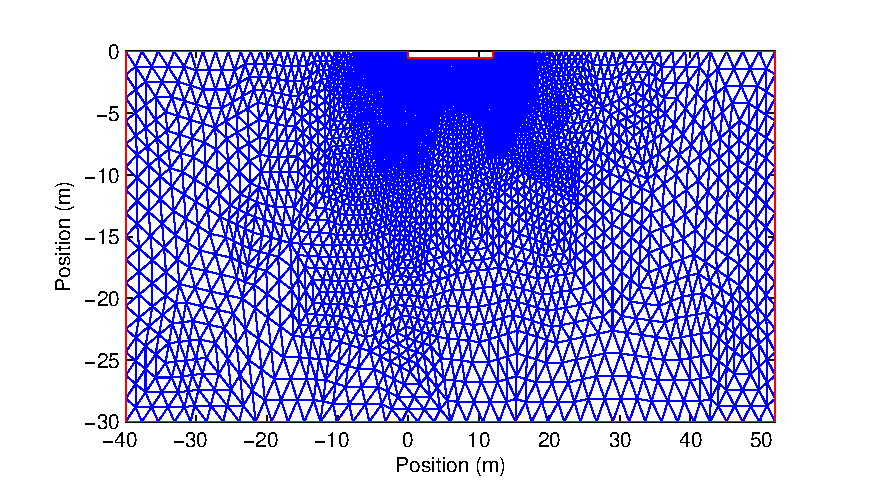
\includegraphics{images/trifoundation.eps}
\caption{Definitionsmängd samt triangulering berget under grunden.}
\end{figure}


\begin{figure}
\centering
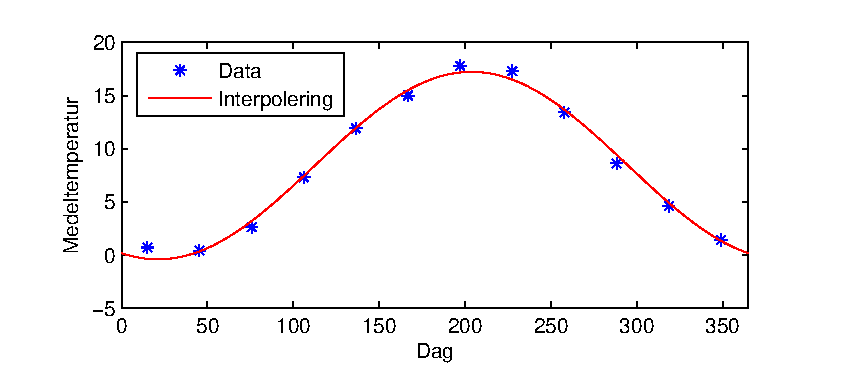
\includegraphics{images/meantemperature.eps}
\caption{
Medeltemperaturen för göteborg de senaste 20 åren. Punkterna är data tagna från Miljöförvaltningen och linjen är minstakvadratanpassningen som senare använts för att beräkna energiflöden.}
\end{figure}

%Miljöförvaltningen
%http://www4.goteborg.se/prod%5Csk%5Cstatistik%5CstatistikR5.nsf/0/3F002A395ED39AC8C1256D3B00393D0E/$File/3.01.pdf

\subsection{Finita element av inkompressibel fluid}

För att lösa Navier-Stokes ekvationer kan lämpligen en datormodell användas.
Här består denna modell av ett system uppsatt med Galerkins metod.
I denna lösning så begränsar vi dock oss till att enbart behandla statiska flöden
vilket genomförs genom att sätta alla tidsderivator till noll.

För att hantera trycket i \eqref{eq:convection:continuity}-\eqref{eq:convection:energy} används den tidigare nämnda Boussinesq approximation
samt penalty metoden för att göra hastighetsvektorn källfri och uppfylla
kontinuitetsekvationen. Det finns således inget direkt behov av att räkna ut trycket.
Vid användning av många sorters elementtyper som inte uppfyller Babuska-Brezzikriteriet
är detta dessutom nödvändigt då det annars kan bildas oönskade trycknoder. 
En annan möjlighet är att välja divergensfria element. \cite{babuska1973}\cite{segal2011}

Genom penaltymetoden beskrives här trycket som $p$ enligt ekvation
\eqref{eq:femconvection:penalty}. Här är $p_s$ någon form av idealt statiskt
tryck som är önskat. Detta tryck följer Boussinesq approximation. Med dessa
idealiseringar kan differentialekvationerna sättas upp igen. \cite{heinrich88}\cite{taylor79}
Som kan ses så leder den godtyckliga penaltyparametern $\lambda$ till att justera trycket
om hastighetsfältets divergens ej är identiskt noll. I viss litteratur anges 
det att penaltyparametern skall vara i storleksordningen $10^7$ men att den
är väldigt applikationsberoende. En för liten vald penaltyparameter leder till att
trycket inte elimineras. Andra problem uppstår vid en för stor parameter. Ekvationssystemet
kan bli svårlöst och få stabilitetsproblem när parametern blir
för stor i jämförelse med de andra delarna i differentialekvationen.\cite{reddy93}\cite{roy05}\cite{basak04}\cite{segal2011}

\begin{equation}
\label{eq:femconvection:penalty}
p = p_s - \lambda\nabla\cdot\mathbf{v}
\end{equation}

\noindent
Fortsatt skall trycket deriveras med avseende på de rumsliga variablerna vilket möjliggör
att eliminera trycket från differentialekvationerna. Dessa deriveringar kan ses i ekvation
\eqref{eq:femconvection:partx} samt \eqref{eq:femconvection:partz}. Notera att det statiska trycket
$p_s$ ej beror på $x$ vilket resulterar i att derivatan är noll.

\begin{equation}
\label{eq:femconvection:partx}
\frac{\partial p}{\partial x} = \frac{\partial p_s}{\partial x} -
\frac{\partial}{\partial x} \lambda\nabla\cdot\mathbf{v} = -
\frac{\partial}{\partial x} \lambda\nabla\cdot\mathbf{v}
\end{equation}

\begin{equation}
\label{eq:femconvection:partz}
\frac{\partial p}{\partial z} = \frac{\partial p_s}{\partial z} -
\frac{\partial}{\partial z} \lambda\nabla\cdot\mathbf{v} =
-g\rho_0 - \frac{\partial}{\partial z} \lambda\nabla\cdot\mathbf{v}
\end{equation}

\noindent
Detta förs in i momentekvationerna vilket ger ekvationerna \eqref{eq:femconvection:u} -
\eqref{eq:femconvection:T}. Här är det ekvationssystem som syftar att lösas.

\begin{equation}
\label{eq:femconvection:u}
\mathbf{v}\cdot\nabla u =
\frac{\lambda}{\rho_0}\nabla\cdot\mathbf{v} +
\nu\Delta u
\end{equation}

\begin{equation}
\label{eq:femconvection:w}
\mathbf{v}\cdot\nabla w =
\frac{\lambda}{\rho_0}\nabla\cdot\mathbf{v} + \nu\Delta w +g\beta(T-T_0)
\end{equation}

\begin{equation}
\label{eq:femconvection:T}
\mathbf{v}\cdot\nabla T = \alpha\Delta T
\end{equation}

\subsubsection{Svag formulering}

En finita elementlösning med Galerkins metod kräver att problemet reduceras till
ett ekvivalent variationsproblem. Här söks $T\in\Phi$, $u\in\Phi$ och
$w\in\Phi$ som uppfyller ekvation \eqref{eq:femconvection:variation}. Här
betecknar brackets skalärprodukt, $\mathbf{L}$ är differentialoperatorn
som betecknar systemet av differentialekvationer som $\mathbf{L}(T,u,w) = 0$.
$\Phi$ är rummet av alla testfunktioner $\phi$ som är kontinuerliga i
definitionsmängden $\Omega$ samt vars derivator är bitvis kontinuerliga på randen
$/Gamma$. De måste även vara $L^2$ integrabla.

\begin{equation*}
\label{eq:femconvection:variation}
\langle \mathbf{L}(T,u,w), \phi \rangle = 0\mbox{,  } \forall \phi \in \Phi
\end{equation*}


\subsection{Datorsimulering av ofrivillig ventilation}




%Resultat
\chapter{Resultat}

I detta kapitel presenteras de resultat som erhållts med hjälp av metodiken i föregående kapitel. De olika delresultaten redogörs i samma ordning som de gjordes förut och kapitlet avslutas med en sammanställning av de individuella bidragen till värmeflödena.

\section{Kvantitativ beskrivning av energiflöden}

Genom att beräkna storlekarna av energiflödena genom byggnadens olika delar kan vi se var energiflödena är som störst vid olika väderförhållanden. Vi har valt att titta på en klar dag i mitten av april då solinstrålningen når en topp vid $\unit[640]{W/m^2}$ och solen är uppe i 14 timmar. Dygnets temperatur varierar mellan $\unit[6]{^\circ C}$ och $\unit[9]{^\circ C}$ och vinden är runt $\unit[10]{m/s}$. Enligt väderstatistik från SMHI\cite{SMHIdata} bör detta vara en rimlig dag med väldigt bra väder vid den valda tiden på året.

Vi vald en dag med fint väder eftersom energiflödena då är små och kan de förbättras när de är små, kan de också förbättras när de är stora. Att vi valde en dag i april beror på att det fortfarande är under eldningssäsongen, det vill säga den tid på året då man fortfarande värmer upp huset. Eldningssäsongen för fastigheten på Walleriusgatan är ungefär från början oktober till slutet av april. Under sommaren sker ingen uppvärmning.

\section{Konstanta energiflöden}

En del av energiflödena är relativt konstanta sett till en längre tidsperiod. Dessa är främst värme från elektriska apparater, så som kylskåp och datorer, människors kroppsvärme och varmvattencirkulation. Även kylningen från husets grund anses vara konstant.

Väldigt liten del av den energi som förbrukas i en elektrisk apparat blir till något annat än värme. Därför låter vi det energiflödet motsvaras av fastighetens energiförbrukning. Den kan läsas av kontinuerligt och på så sätt reglera aktivt tillförd energi\footnote{Aktivt tillförd energi: Den energitillförsel som kan regleras och tillförs via radiatorerna.}.

Människornas utstrålade kroppsvärme kan beräknas genom att de antas vara svartkroppar. Stefan-Boltzmanns lag säger då att utstrålade energi per yt- och tidsenhet är $j=\sigma T^4$, där $T$ är temperaturen och $\sigma=\unit[5.6705\cdot 10^8]{Wm^{-2}K^{-4}}$ \cite{physicshandbook}. På samma sätt beräknas den energi som strålas in mot kroppen från omgivningen. Nettostrålningen från en människa kan då ses i ekvation \eqref{eq:constantsources:stefan} där $T_k=37^{\circ}C=310K$ är kroppstemperaturen och $T_r=20^{\circ}C=293K$ är rumstemperaturen. Multiplicerat med en människas area, ungefär $\unit[2]{m^2}$, fås en nettoeffekt på $\unit[211]{W}$. I själva verket reduceras denna effekt av en rad faktorer. Exempelvis är hudens temperatur lägre än kroppstemperaturen samtidigt som klädesplagg reducerar effektutstrålningen något. Det är allmänt vedertaget att man kan sätta nettoeffekten till ungefär $\unit[50-100]{W}$.

\begin{equation}
\label{eq:constantsources:stefan}
j=\sigma \left( T_k^4 - T_r^4 \right)
\end{equation}
\noindent
I huset cirkulerar hela tiden varmvattnet för att alltid kunna tillgodose de boendes behov av varmvatten utan dröjsmål. Efter en tur i systemet sjunker temperaturen på varmvattenet med tre grader. Detta motsvarar en energitillförsel till fastigheten på \textcolor{red}{??} $\unit[]{W}$.

Grunden huset står på har en randtemperatur på ungefär $6^{\circ}\mbox{C}$ från marken. Den kan antas vara konstant då huset grund ligger en bit ned under marken. Enligt SLU, Sveriges Lantbruksuniversitet, kan marktemperaturen antas vara konstant från $\unit[1,6]{m}$ under markytan \cite{SLU}. Deras data kommer från Uppsala vilket borde vara jämförbart med Göteborg. Huset står på en grund som består av ett luftgap och sedan $\unit[0,25]{m}$ betong. Längst ned i huset finns en källare som är ouppvärmd \textcolor{red}{??}. Det energiläckage som då blir genom husets grund ned i marken kan beräknas uppgå till \textcolor{red}{??} $\unit[]{W}$.


\subsection{Energiflöde genom väggar}

\input{sections/steadystatewalls}

\input{sections/transientwalls}

\input{sections/humiditywalls}

\input{sections/leakagewalls}


\subsubsection{Solstrålning genom fönster}

Exempel på resultat från beräkningar på solstrålning genom fönster. Beräknat via trial.m i code-mappen.

I figur \ref{fig:vinklar120401} ses de relevanta vinklar som bildas av solens position den första april, 2012. Den blå linjen i figuren representerar solens vinkel relativt ett fönsters normal (då denna pekar i horisontell sydlig riktning) och kan användas för att uppskatta effekten som solinstrålning bidrar till. Om solens intensitet antas vara konstant $\unit{200}{W/m^2}$ beräknas denna effekt motsvara vad som visas i figur \ref{fig:effekt120401}. Här antas fönstrets area uppgå till $\unit{1.5}{m^2}$, g-värdet för normal solstrålning är ? och värdet p i koden sätts till ?, ty fönstren i den avsedda byggnaden är av typ treglas utan ytbeläggningar.

\begin{figure}[hpbt]
\centering
\includegraphics[scale=1]{images/angles120401.eps}
\caption{\label{fig:vinklar120401} Beräknade vinklar vid Walleriusgatan den första april 2012, tid i UTC}
\end{figure}

\begin{figure}[hpbt]
\centering
\includegraphics[scale=1]{images/effekt120401.eps}
\caption{\label{fig:effekt120401} Beräknad effekt genom ett fönster vars normal pekar i horisontella sydriktningen, den första april 2012. Solens intensitet tas konstant till 200 W/m$^2$}
\end{figure}


\section{Energiflöde genom grunden}

\input{sections/steadystatefoundation}

\input{sections/transientfoundation}



\section{Konstanta energiflöden}

En del av energiflödena är relativt konstanta sett till en längre tidsperiod. Dessa är främst värme från elektriska apparater, så som kylskåp och datorer, människors kroppsvärme och varmvattencirkulation. Även kylningen från husets grund anses vara konstant.

Väldigt liten del av den energi som förbrukas i en elektrisk apparat blir till något annat än värme. Därför låter vi det energiflödet motsvaras av fastighetens energiförbrukning. Den kan läsas av kontinuerligt och på så sätt reglera aktivt tillförd energi\footnote{Aktivt tillförd energi: Den energitillförsel som kan regleras och tillförs via radiatorerna.}.

Människornas utstrålade kroppsvärme kan beräknas genom att de antas vara svartkroppar. Stefan-Boltzmanns lag säger då att utstrålade energi per yt- och tidsenhet är $j=\sigma T^4$, där $T$ är temperaturen och $\sigma=\unit[5.6705\cdot 10^8]{Wm^{-2}K^{-4}}$ \cite{physicshandbook}. På samma sätt beräknas den energi som strålas in mot kroppen från omgivningen. Nettostrålningen från en människa kan då ses i ekvation \eqref{eq:constantsources:stefan} där $T_k=37^{\circ}C=310K$ är kroppstemperaturen och $T_r=20^{\circ}C=293K$ är rumstemperaturen. Multiplicerat med en människas area, ungefär $\unit[2]{m^2}$, fås en nettoeffekt på $\unit[211]{W}$. I själva verket reduceras denna effekt av en rad faktorer. Exempelvis är hudens temperatur lägre än kroppstemperaturen samtidigt som klädesplagg reducerar effektutstrålningen något. Det är allmänt vedertaget att man kan sätta nettoeffekten till ungefär $\unit[50-100]{W}$.

\begin{equation}
\label{eq:constantsources:stefan}
j=\sigma \left( T_k^4 - T_r^4 \right)
\end{equation}
\noindent
I huset cirkulerar hela tiden varmvattnet för att alltid kunna tillgodose de boendes behov av varmvatten utan dröjsmål. Efter en tur i systemet sjunker temperaturen på varmvattenet med tre grader. Detta motsvarar en energitillförsel till fastigheten på \textcolor{red}{??} $\unit[]{W}$.

Grunden huset står på har en randtemperatur på ungefär $6^{\circ}\mbox{C}$ från marken. Den kan antas vara konstant då huset grund ligger en bit ned under marken. Enligt SLU, Sveriges Lantbruksuniversitet, kan marktemperaturen antas vara konstant från $\unit[1,6]{m}$ under markytan \cite{SLU}. Deras data kommer från Uppsala vilket borde vara jämförbart med Göteborg. Huset står på en grund som består av ett luftgap och sedan $\unit[0,25]{m}$ betong. Längst ned i huset finns en källare som är ouppvärmd \textcolor{red}{??}. Det energiläckage som då blir genom husets grund ned i marken kan beräknas uppgå till \textcolor{red}{??} $\unit[]{W}$.


\section{Tidskonstanter}

% Eliminerat avsnitt, kan tas bort

\section{Sammanfattning av energiflöden: free-running temperature}




%Diskussion
\chapter{Diskussion}

Under vår undersökning av hur byggnadens energiflöden påverkas av olika 
väderparametrar har vi stött på problem ibland varit tvungna att göra grova 
approximationer. Här diskuterar vi problemen närmare och utvecklar resonemanget om
 vilka fel de kan ha gett upphov till. Vidare kommer några förslag på hur arbetet kan
 appliceras för att minska energiflödet ut ur den aktuella byggnaden på Walleriusgatan 
 likväl som mer allmänt. Slutligen ges några förslag på hur man kan gå vidare och 
 vidareutveckla det här arbetet. 
  
\section{Felkällor}

Onoggrannheten i beräkningsmodellerna.

Ingen hänsyn till att väggarna tar åt sig fukt vid blött väder och därmed ändrar egenskaper (t.ex. ändras värmeledningsförmågan). 

Alla approximationer – hur stora fel.

% Koppla mot avgränsningar.
% Vad har de här avgränsningarna lett till för fel.

\section{Problem som vi stött på}

I början av arbetet hoppades vi att fastighetens väderstation skulle kunna tillhandahålla väderdata som vi kunde använda för att sätta upp statistiska modeller. 
Ganska snart insåg vi dock att detta inte skulle bli verklighet och vi planerade istället att sätta upp analytiska modeller. 
Senare visade sig dock att statistiken hade varit bra för att närmare kunna undersöka hur stor inverkan olika väderparametrar har vid just fastigheten på Walleriusgatan. 
Detta fick istället lösas med statistik från SMHIs hemsida, som dock visade sig vara något otillräcklig.

För att sätta upp de analytiska modellerna behövdes också värden för ett antal materialkonstanter för luft och för tegel. 
Dessa beror dock av en eller flera väderparametrar så som tryck, temperatur och fukt och således är det tveksamt om de överhuvudtaget bör kallas konstanter. 
Det visade sig dock vara mycket svårt att få fram tillförlitlig och tillräckligt högupplöst data som visade detta än mindre uttryck av ekvationskaraktär. 
Vid diskussion med sakkunniga fick vi uppfattningen att det finns en tydlig konsensus inom branchen vad som är relevant och inte, men ingen tydlig dokumentation på området.

Konvergens. Svårt att få våra datamodeller att konvergera. 

Svårt att få exakta värden på kostnader efter som vi är tredje part.


\section{Jämförelse med andra energibesparande åtgärder}

Det finns flera olika energibesparande åtgärder att överväga. Innan något av alternativen implementeras måste det klargöras vilka kostnader, mervärden och sidoeffekter olika system ger samt hur de kan utnyttjas maximalt. De finns lösningar som lämpar sig bättre och sämre för specifika byggnader. I det här avsnittet kommer en diskussion föras angående fyra alternativ till det momentant väderbaserade system rapporten i övrigt undersöker.
Som kan ses i resultatet påverkar vädret högst väsentligt energiflödet genom byggnaden. Enligt avsnittet \ref{resultsfreerunning} beror det främst på vind och solinstrålning och dess effekter fördröjs inte av trögheten i väggarna, vilket var en av utgångspunkterna för arbetet. För att kunna reglera enbart på redan insamlad data behöver det finnas en fördröjning innan vädret påverar inomhusklimatet för att reglersystemet ska hinna med. Solinstrålningen värmer direkt genom fönster, och vinden går in igenom otätheter och för på så sätt in kallare luft i byggnaden utan fördröjning.

All energi som används till bostadsuppvärmning enligt fastighetens energideklaration\cite{energideklaration} antas ligga under vinterhalvåret, då uppvärmning förekommer. Det antas inte försvinna energi till kyla under sommarhalvåret, då fastigheten idag inte har något kylsystem.

\subsection{Tilläggsisolering}
Våra beräkningar visar att väggen inte absorberar tillräckligt mycket energi för att det ska vara värt att inte isolera den. Se figurer i avsnitt~\ref{sec:steadystatewall}.
När man gjorde en omfattande renovering i slutet av 1980-talet byggde man en yttre tilläggsisolering, med tio centimeter mineralull på den norra sidan\cite{arsredovisning}, som motsvarar $\unit[26]{\%}$ av husets yta utåt, grunden borträknad. Isoleringen gav en sänkte U-värdet med en fjärdedel. Norrväggen fick då ett lägre U-värde medan syd- och västväggarna fortfarande hade ett relativt högt, se tabell {tbl:uvalue}.
Dessa differenser belyser var byggnaden är dåligt isolerad och det är lämpligt att göra förbättningar, till exempel där U-värdet ligger över ett.

En isolering av både syd- och västväggarna är en isolering av en yta om 212 $\unit{m^2}$, som rent i och med isolering skulle få ett bättre U-värde. Det motsvarar $\unit[21,8]{\%}$ av fastighetens ytan där energi kan ledas ut, se tabell \ref{tbl:uvalue}.
En tilläggsisolering kan göras på två olika sätt, inifrån eller utifrån. Med båda metoderna finns för samt nackdelar. Båda metoderna innebär också betydande insatser i fastigheten. Det finns dock mervärden att ta under beaktande. 

\paragraph{Sidoeffekter och besparingar}
Fasader behöver med jämna mellanrum renoveras, och i samband med tilläggsisolering kan det vara lämpligt att även fasadrenovera. Svenskt tegel har en ungefärlig livslängd på 50 år\cite{magnus}, dock ska tegelfasaden ha renoverats med ny impregnering i samband med renoveringen 1988. Teglet i fastigheten har troligtvis även en bättre livslängd än 50 år,  då tegel höll högre kvalitetet när huset byggdes och då handlar det om en livslängd på ungefär 100 år. Det största mervärdet utifrån det som initierade det här projektet är att temperaturerna i bostäderna blir jämnare, se figur~\ref{fig:energyflow_stst} och \ref{fig:wall_dec}. Det beror på att fasaden inte fungerar så bra som att spara energi i från den varmare till den kallare delen av dygnet. Dess buffrande egenskaper är inte så stora som man vill tro.

\paragraph{Tilläggsisolering utifrån}
En tilläggsisolering utifrån är ett ingrepp som medför en stor kostnad. Områdena som bedöms vara lämpliga att tilläggsisolera är alla väggar med tegelyta, då de inte har någon tilläggsisolering sedan tidigare och U-värdet skulle då kunna sänkas på samma sätt som norrsidan när den isolerades. U-värdet för hela fastigheten skulle då kunna sänkas från 0,6 till 0,4. Men då tilläggsiolering är en betydande investering måste mervärden och andra kostnader som kan tänkas uppstå tas under beaktande. Då alla fasader med jämna mellanrum behöver renoveras kan det vara lämpligt att göra isoleringen i samband med detta. Vissa kostnader skulle då kunna minskas, till exempel den för uppsättande av byggnadsställningar.

\paragraph{Tilläggsisolering inifrån}
En tilläggsisolering inifrån innebär ett ingrepp i lägenheterna och förutom den direkta nackdelen att det stör dem som bor där medför det också att lägenheterna blir något mindre. Huruvida de boende behöver kompenseras ekonomiskt eller i form av alternativt boende i samband med renoveringen har inte tagits ställning till. Vidare blir ingreppet inte lika komplett som vid isolering utifrån, eftersom det inte går att isolera där innerväggar och golvplan ansluter till ytterväggen och bildar köldbryggor utåt. Den beräknade ytan att isolera blir nedåt hälften mot att isolera utifrån. Detta gör den troligen själva isoleringen mindre kostsam, men det har inte undersökts närmare.

\subsection{Termostater på radiatorererna}
Den tredje åtgärden som undersökts är styrning av rumstemperatur via termostater på radiatorerna. I dagsläget regleras flödet manuellt via vred under elementen. De ställs in av fastighetsskötaren och kan regleras om bostadsrättsinnehavaren är missnöjd med inomhusklimatet. Elektriska termostater finns i olika varianter, men det är främst en ett koncept från Danfoss som undersökts. Det finns i två varianter vilka går att implementera på i princip alla befintliga uppvärmningssystem. Temperatur ställs in i önskat antal grader, i det billigare systemet direkt på termostaterna via en lite lcd-display, eller i det dyrare systemet med en större färgdisplay som är ansluten trådlöst till en huvudenhet. Båda systemen kan automatiskt bryta tillförseln av energi vid tillfälliga kyltoppar, till exempel vid vädring. Det går genom systemet att hålla lägre temperatur i vissa rum, till exempel sovrum. Systemen kan programmeras att ta hänsyn till solinstrålning genom fönster och att sänka temperaturen under dagen, natten eller semestern. Enligt resultaten i avsnitt~\ref{resultsfreerunning} vet vi att kompensering för solinstrålningen kan ge en stor energibesparing.

\paragraph{Sidoeffekter och besparingar}
En negativ bieffekt är att energianvändningen kan öka om det finns tillräcklig med energi i systemet och de boende vill ha varmare än vad som i dagsläget erbjuds, vilket leder till att det går åt mer energi än tidigare. Det är lätt att begränsa temperaturintervallet för alla, men det kan skapa irritation hos de boende om de upplever fel temperatur och inte kan ändra, när systemet ska klara det. I samband med ett system där de boende själva kan reglera temperaturen implementeras bör man informera de boende på ett attraktivt sätt – meningen är ju att både kostnaden ska sjunka, samt att miljöpåverkan ska minskas. Höjs då temperaturen i lägenheterna blir så inte fallet utan det börjar istället kosta mer i både uppvärmning och förslitning av pumpar. \cite{viivilla}

\subsection{Prognosstyrning}
Prognosstyrning är en möjligheten för att styra inomhustemperaturen efter vädret, vilket skulle kunna vara ett alternativ till styrning efter väderstationen för byggnaden som har studerats.
Fördelarna med prognosstyrning jämfört med att styra direkt mot väderstationen är att de flesta markanta väderpåverkningarna är momentana, det vill säga att det inte sker någon fördröjning innan de påverkan inomhusklimatet. Då krävs framförhållning för att kunna ta hänsyn till dessa vilket kan ges av prognosstyrning. Sveriges meterologiska och hydrologiska institut, SMHI, står för prognoserna som skickas till systemet, vilket i sin tur har installerats av deras samarbetspartner. En prognos skickas egentligen aldrig, utan det som skickas är en styrsignal som baseras på väderprognoser samt data om byggnadens energibalans som skickas till styrsystemet. Styrsystemet försöker sedan optimera energiåtgång och boendekomfort efter de givna värden.

\paragraph{Sidoeffekter och besparingar}
SMHI påstår att deras prognosbaserade system ger kostnadsbesparingar på 5 till 10 \% på uppvärmningen. Att förutsäga exakt hur mycket är väldigt svårt då deras modell angående vilka parametrar styrningen beror på är kommersiell och således inte delges allmänheten. Antydningar från vårt möte med SMHI menade att den här fastigheten inte låg i den övre delen av skalan, men det beror ju helt på hur olika parametrar viktas, och för en korrektare bedömning kräver troligtvis att man har för avsikt att köpa det.

\subsection{Ekonomiska uppskattningar kring de olika åtgärderna}
Vilka ekonomiska förutsättningar som krävs för de olika åtgärden kan bara uppskattas då vi inte har haft befogenheter att begära in riktiga offerter från bygg- och installationsföretag.

För att beräkna kostnaderna användes genomgående en förenklad version av payoff-metoden, som visar hur många år det tar innan en investering betalar av sig. Metoden tar inte hänsyn till att det är olika stora investeringar, och det framgår således inte vilken metod man kan spara mest pengar på utan vilken som lönar sig snabbast. Det finns inget restvärde för någon av investeringarna. Beräkningarna har gjorts för mest positiva samt mest negativa möjliga utfall, vilket ger ett spann på ett antal år. Förenklingarna leder till att varken kalkylräntor eller en eventuell ränta i det fallet investeringen måste finansieras med ett banklån tas med i beräkningen. Den enklaste formen ges enligt ekvation\cite{ind.ek}

\begin{equation} \label{eq:payback}
\text{Antalet år}=\frac{\text{Grundinvestering}}{\text{Sparat belopp per år}}
\end{equation}

Antalet år det tar innan en investering betalar sig enligt \eqref{eq:payback} ges i tabell \ref{tbl:payback} nedan.

\begin{table}[hbtp]
\centering
\caption{Paybacktid för olika investeringar}
\label{tbl:payback}

\begin{tabular}
{|l|r|r|}
\hline
\textbf{Investering} & \textbf{Minimal paybacktid[år]} &{\textbf{Maximal paybacktid[år]}} \\
\hline
Tilläggsisolering & 8,7 & 52,2 \\
\hline
Termostater & 2,9 & 12,8 \\
\hline
Prognosstyrning &  1 & 2,9 \\ 
\hline
Väderstation & 1,7 & 5,2 \\
\hline

\end{tabular}
\end{table}

\paragraph{Isolering}
Vi har inte räknat på en isolering inifrån då det inte har varit möjligt att få en offert eller prisförslag på ett sådant arbete. Det är inte heller säkert att det är möjligt att göra på grund av de boendes preferenser. Genom en internetbaserad förfrågningstjänst en tjänst på internet fick vi visserligen kontakt med ett byggföretag som hävdade att de skulle kunna göra arbetet för 200 000 kronor, vilket enligt lite uppskattningar över kostnader för material, arbetskraft och byggställningar framstår som väldigt billigt. Dock har vi en uppskattad besparingsmöjlighet på 25 \%, vilket ger payoff-tiden dryga 10 år, vilket för en sådan typ av investering får anses vara låg. Kostanden 200 000 kronor är troligtvis för låg, då det endast var en bedömning utifrån ytan som skulle isoleras samt att det var upp till 8 våningar över mark. En seriös offertförfrågning skulle ge en rättvisare approximation, men det bedömdes att de befogenheterna saknades inom projektet.

\paragraph{Termostater}
Det bästa fallet är framräknat utan avseende på varken installationskostnad eller räntor på kapital som måste lånas in. Sämsta fallet framräknat med en installationskostnad lika hög som materialet, vilket bör kunna motsvara ett rimligt scenario. En investering av det här slaget bör ha en avskrivningstid på fem år, vilket är intressant att jämföra payback-tiden mot. Materialet i sig skulle kosta föreningen knappa 100 000 kronor, och med en besparing på upp till 46 \% \cite{danfoss} per år blir payback-tiden under tre år. En payback-tid på runt halva uppskattade avskrivningstiden är en bra investering. Det är dock ett orimligt scenario, men räknat på dubbla kostnaden och endast 25 \% besparing är Paybacktiden tolv år, vilket är tilltaget i överkant. Rimlig Paybacktid skulle kunna vara runt 5-6 år, med den dyrare varianten av systemet. Det finns också möjlighet att sätta in det billigare, utan färgskärmarna. Det ger halva kostnaden, men ger inte samma mervärde och enkelhet till de boende.

\paragraph{Prognosstyrning från SMHI}
Den stora fördelen med SMHIs system för prognosstyrning är SMHIs prismodell. Den innebär att investeringskostnaden ska kunna betala sig inom två år, samt att abonnemangsavgiften inte är högre än maximalt hälften av vad man sparar varje år. Det är således väldigt intressant eftersom man egentligen inte behöver några ekonomiska muskler för att börja använda produkten – även en förening som redan har mycket lån och nästan går med minus kan köpa systemet. Det bidrar till att samtidigt som SMHI kan ta betalt för sina prognoser, så sparar de boende pengar och mindre energi behöver produceras. SMHI lejer ut installationen till sina sammarbetspartners. Systemet är enkelt och lätt att installera, vilket tillsammans med det låga priset bidrar till att göra det attraktivt.

Med, som bäst, endast ett års payback-tid är prognossytrning det alternativet som verkar bäst enligt Payback-metoden. Det är dock känt att payback-metodern inte alltid hittar de största besparingarna. Skulle föreningen investera i systemet, som man enligt SMHI ska kunna få installerat till ett pris som betalar sig inom ett eller maximalt två år \cite{smhi1}\cite{smhi2}, tjänar man efter paybacktiden inte nödvändigtvis speciellt mycket pengar per år. Det är inte en hög procentsats av energiåtgången som sparas, samtidigt som de tar en abonnemangsavgift uppskattningsvis 20-40 \%. \cite{smhi1}\cite{smhi2}

\paragraph{Väderstation}
Beräkningarna för väderstationen är gjorda utifrån inköp av nödvändigt utrustning. För Bostadsrättsföreningen Wallerius är detta inte riktigt relevant då investeringen redan är gjord. I och med beräkningen finns det ändå en möjlighet för att se hur metoden står sig i förhållande till de andra där främst jämförelsen med prognosstyrning är intressant.


\section{Tillämpningar}

De två primära tillämpningarna av det här arbetet är att identifiera energiläckor för att kunna göra sitt hus mer energieffektivt och att låta sitt energiförsörjningssystem vara väderberoende.

Att energieffektivisera sitt hus kan, om man väljer rätt metod, löna sig både ekonomiskt och miljömässigt. Det leder dessutom till mindre fluktuationer i inomhustemperaturen, speciellt om man har stor tröghet i sitt uppvärmningssystem.

Att låta energiförsörjningssystemet bero av väderdata från en vid fastigheten monterad väderstation kräver experimentella mätning på den aktuella fastigheten för att bli implementerbart.
Dessutom kommer direkta eneriflöden, så som solinstrålning och vind, att kompenseras för fördröjt, vilket kan bli ett problem om man har ett långsamt system för uppvärmning. Ett alternativ då är prognosstyrning men de färdiga system som finns på marknaden idag är så pass bra att det inte är av intresse att försöka bygga ett eget, inte ur ekonomisk synvinkel i alla fall.


\section{Rekommendationer till fortsatt arbete}




%Slutsats
\chapter{Slutsats}

%Sammanfattning av resultat

I detta projekt har olika väderparametrars effekt på inomhusklimat och energiåtgång studerats.
Det har framgått att både solinstrålning och infiltrationsförluster på grund av ofrivillig
ventilation kan leda till stora energibidrag. Inom arbetet har även olika förbättringsåtgärder
studerats. Det har visat sig att energibesparingen för att dra nytta av solens värmande effekt kan ge 17~\% lägre energiåtgång över ett soligt dygn, vilket motsvarar 4~\% energibesparing över alla dygn, klara som molnig. Detta kan jämföras med mängden sparad energi för tilläggsisolering för syd- och västväggarna som uppgår till 17~\% av dagens energiåtgång. Det kan också konstateras att de olika väggarna har olika tidskonstanter vilket man måste ta hänsyn till vid regleringen med olika reglersystem för olika delar i byggnaden. Denna effekt kommer dock att minskas något med en tilläggsisolerad av syd- och västväggarna.

Att ta hänsyn till vinden kommer inte nödvändigtvis leda till en lägre energiförbrukning då vinden har en kylande effekt. När det blåser sjunker inomhustemperaturen under önskad temperatur med dagens system om man inte överkompenserar när det inte blåser. Att ta hänsyn till vinden leder dock till en stabilare inomhustemperatur eftersom man eliminerar vindens temperatursänkning.

%Ekonomiska aspekter
Energibesparande åtgärder utöver den direkta styrningen är möjliga att genomföra. För att gå vidare i processen antingen med termostater till alla radiatorer eller tilläggsisolering av ej isolerade fasader behöver föreningen utarbeta en plan för hur de vill att fastigheten ska vara rustad i framtiden. När fasaden behöver renoveras, samt om man får renovera den behöver också besvaras, för att ge tillräcklig information inför en eventuell energibesparande åtgärd. 

Montering av termostater på elementen är billigare än att tilläggsisolera fasaden och enligt beräkningar samt information från leverantörer är det även mer energibesparande. En annan aspekt är att det tillför mervärde för de boende. De boende vill troligtvis kunna reglera temperaturen själva, och vid försäljning av lägenheter bör det kunna ha ökat värdet på desamma.

I samband med en installation av ett reglersystem bör även elektriska termostater installeras, för att minimera tidskonstanterna och för att ge de boende möjligheten att själva bestämma vilken temperatur de vill ha hemma.

%Bevara frågeställningar
Det det har visat sig vara en god idé att ta hänsyn till olika väderparametrar då
detta kan ge en markant besparing under rätt förutsättningar. Självklart är
besparingen olika beroende på fastighetens egenskaper och fastighetens geografiska läge.

%Vad kunde vi inte besvara
Det var svårt att med någon större noggrannhet kvantifiera storleken på de olika energiflödena. Vi
anser dock att våra approximationer ger en god uppfattning om hur stora energiflödena är i förhållande
till varandra. För att få veta exakta värden skulle det vara nödvändigt att implementera de olika
förbättringarna i fastigheten och mäta hur mycket energi som sparats. Alternativt skulle
bättre modeller kunna ge en exaktare bild. Problemet med det är att mer komplexa modeller tenderar att
bli mer beräkningsintensiva.



%\input{}


%---
\newpage
\clearpage
\addcontentsline{toc}{chapter}{Referenser}
\bibliography{ref}{}
\bibliographystyle{plain}
\newpage
\appendix

\section{Formler för linjära triangulära element}


\newpage
\chapter{Matlab-kod}
\label{sec:mcode}

%\rhead{Appendix \ref{sec:mcode}}

\section{Beräkning av solens position}\label{app:sunposition}

\lstinputlisting{../code/sun/sunposition.m}

\section{Beräkning av effekt genom fönster}\label{app:sunwindows}
\lstinputlisting{../code/sun/angletheta.m}

\lstinputlisting{../code/sun/gvalue.m}

\lstinputlisting{../code/sun/effekt.m}

\section{Finita element av energiflöde genom grund}\label{app:femfoundation}

\lstinputlisting{../code/pdesolver/groundheatfemtransientanalys.m}

\lstinputlisting{../code/pdesolver/triarea.m}

\lstinputlisting{../code/getMeanTemp.m}

\lstinputlisting{../code/pdesolver/laplacestiff.m}


%Add a new page between each appendix

\end{document}
